    
\chapter{The 10 Major Aspects of Japanese}

\begin{center}
\begin{Large}
第7課: The 10 Major Aspects of Japanese 
\end{Large}
\end{center}
 
\par{ Japanese ( \emph{Nihongo }日本語) is a major world language. Depending on how one defines a language, it may be ranked as the eighth to the tenth most spoken language. Japanese is predominantly spoken in Japan. In Japanese, "Japan" is called 日本, which is usually pronounced as \emph{Nihon }にほん, but it may also be pronounced as \emph{Nippon }にっぽん. \emph{Nippon }is favored in formal settings, but in reality, \emph{Nihon }and \emph{Nippon }are both used in many of the same situations. The country is formally called \emph{Nipponkoku }日本国 (the nation of Japan). }

\par{ The country of Japan is said to have been founded by Emperor Jimmu ( \emph{Jimmu Ten'nō }神武天皇) on February 11, 660 B.C. Its national flag is called the \emph{Hinomaru }日の丸, a reference to it being the land of the rising sun. In this lesson, you will learn about ten of the most important aspects of Japanese. In doing so, the mysteries of Japanese grammar that will be unraveled in the lessons that follow won't be so mysterious after all. }

\par{ Before delving into what Japanese is, let's first address one concern you've likely had thus far: how to say basic everyday expressions. Below are some of those most important phrases that you can use with Japanese speakers. }

\begin{itemize}

\item Good morning: \emph{O-hayō gozaimasu }おはようございます \hfill\break

\item Good afternoon\slash Hello: \emph{Kon'nichi wa }こんにちは \hfill\break

\item Good evening: \emph{Komban wa }今晩は 
\item Good night: \emph{O-yasumi-nasai }お休みなさい 
\item How are you doing?: \emph{O-genki desu ka? }お元気ですか 
\item Nice to meet you: \emph{Hajimemashite 初めまして }
\item Thank you: \emph{Arigatō gozaimasu }ありがとうございます 
\item Yes: \emph{Hai }はい 
\item No: \emph{Iie }いいえ 
\item I'm sorry\slash Excuse me: \emph{Sumimasen }すみません 
\end{itemize}
 The ten aspects that are to be studied in this lesson are as follows: 
\begin{enumerate}

\item The Sounds 
\item A Mixed Script 
\item Word Order \hfill\break

\item Parts of Speech 
\item Agglutination 
\item Speech Styles 
\item Spoken vs Written Language 
\item Etymology 
\item Language Isolate 
\item Dialects 
\end{enumerate}
      
\section{I: The Sounds}
 
\par{ Words are composed of sounds, and every language has its own set of rules that govern how sounds come together to make words. These rules are collectively referred to as the \textbf{phonology }of a language. How sounds simply sound is referred to as the \textbf{phonetics }of a language. }

\begin{center}
\textbf{The Vowels }
\end{center}

\par{ A \textbf{vowel }is a \emph{speech sound made by vibrating the vocal colds without obstructing airflow from the lungs }. In Japanese, there are only five vowels: \slash a\slash , \slash i\slash , \slash u\slash , \slash e\slash , and \slash o\slash . However, they aren't exactly like their English counterparts. To learn how they differ, we need to learn more about what vowels are. }

\par{ \textbf{High vowels }are made with the tongue raised high. Oppositely, \textbf{low vowels }are made with the tongue lowered. \textbf{Front vowels }are made by placing the tongue as close to the front of the mouth as possible. Oppositely, \textbf{back vowels }are made by placing the tongue as far back in the mouth as possible. \hfill\break
}

\par{\textbf{Chart Note }: The diagram below maps out the vowels of Japanese in a vowel space that is meant to represent the dimensions of height and forwardness in the mouth. The further left you go, the closer your tongue is to the front of the mouth. The further right you go, the father your tongue is from the front of the mouth. The further up you go, the higher up the tongue is. The further down you go, the lower the tongue is. }

\begin{figure}[h]
\centering

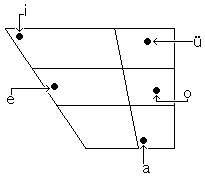
\includegraphics[width=0.9\textwidth]{figs/第01章/第7課:_10majoraspects_fig/Vowel_chart.png}

\end{figure}
 
\par{ The vowel \slash a\slash  is made by with the tongue low but central in the mouth. It is more like the "a" sound found in British English or Spanish. The vowel \slash i\slash  is made with the tongue raised high in the front of the mouth. The vowel \slash u\slash  is also a high-vowel, but it's made with the tongue in the back of the mouth. In the diagram above, it is marked with a diaeresis (two dots) to indicate that it is not made while rounding the lips like its English counterpart. The vowels \slash e\slash  and \slash o\slash  are made with the tongue at the center of the mouth. Whereas \slash e\slash  is made by placing the tongue closer to the front, \slash o\slash  is made by placing the tongue back in the mouth. }

\par{\textbf{Curriculum Note }: Various things can happen phonetically to vowels in Japanese. They may become elongated, nasalized, and even devoiced. To learn more about these processes, see Lesson 365. }

\begin{center}
\textbf{The Consonants }
\end{center}

\par{ In Lesson 2  , we learned about the various consonant sounds of Japanese. A \textbf{consonant }is \emph{a speech sound made by obstructing the airflow from the lungs in some manner }. }

\par{ Consonants come in four broad categories: unvoiced, voiced, palatalized, and nasal. Unvoiced consonants are made by not vibrating the vocal cords. Voiced consonants are made by vibrating the vocal folds. Palatal consonants are made by placing the body of the tongue against the hard palate of the mouth. Lastly, nasal consonants are made by redirected some of the air exhaled from the lungs through the nose. }

\begin{itemize}

\item \textbf{Unvoiced Consonants }( \emph{Museion }無声音): \slash k\slash , \slash s\slash , \slash sh\slash , \slash t\slash , \slash ts\slash , \slash ch\slash , \slash h\slash , f\slash , \slash p\slash . 
\item \textbf{Voiced Consonants }( \emph{Yūseion }有声音): \slash g\slash , \slash z\slash , \slash j\slash , \slash d\slash , \slash dz,\slash  dj\slash , \slash b\slash , \slash n\slash , \slash m\slash , \slash r\slash , \slash y\slash , \slash w\slash . 
\item \textbf{Palatal Consonants }( \emph{Yō'on }拗音): \slash ky\slash , \slash gy\slash , \slash sh\slash , \slash j\slash , \slash dj\slash , \slash hy\slash , \slash py\slash , \slash by\slash , \slash ry\slash , \slash y\slash . 
\item \textbf{Nasal Consonants }( \emph{Bion }鼻音): \slash n\slash , \slash ny\slash , \slash m\slash , \slash my\slash , \slash N\slash . 
\end{itemize}

\par{ There is some overlap between these categories, but this is only natural. The categorization of the consonants above does not take into account variations of the same consonant (allophones). To learn more about allophones and the articulation of each kind of consonant, see Lesson 366. }

\par{ You may remember the terms \emph{seion }清音, \emph{dakuon }濁音, \emph{handakuon }半濁音, and \emph{yō'on }拗音 when we learned about \emph{Kana }仮名. However, they don't 100\% match with the terms above because they describe how sounds have been traditionally categorized. }

\begin{itemize}

\item Any consonant in the Table of 50 Sounds (Goj \emph{ū }onzu 五十音図) is a seion 清音. 
\item A consonant written with a \emph{dakuten }゛is a \emph{dakuon }濁音. It excludes other sounds that vibrate the vocal folds such as vowels, \slash n\slash , \slash m\slash , \slash r\slash , \slash y\slash , and \slash w\slash . 
\item A consonant written with a \emph{handakuten }゜is a \emph{handakuon }半濁音. This term only refers to \slash p\slash , which phonetically is no different other than unvoiced consonants. 
\item A consonant written with a small y- \emph{kana i }s a \emph{yō'on }拗音. This term is the Japanese equivalent of "palatal sound." 
\item Another word you may encounter is \emph{bidakuon }鼻濁音, which refers to pronouncing \slash g\slash  as \slash ng\slash . 
\end{itemize}

\begin{center}
\textbf{The Mora } 
\end{center}

\par{ Unlike English, the basic syllabic structure in Japanese is a mora-based system. A \textbf{mora } \emph{is a unit of sound that is equivalent to a single beat }. Each "beat" is conceptualized as being equal in length, and each beat is assigned a high or low pitch. }

\par{ In reality, morae are not always exactly equal in length, but this is how they are conceptualized. This is then reflected in the writing system. \emph{Kana }仮名 isn't a syllabary. Rather, it's a moraic system which denotes separate characters to each sound (combination) that can be treated as a mora in Japanese. This includes the moraic consonant \slash N\slash , which is written in \emph{Kana }仮名 as ん・ン. }

\par{ The moraic sound system helps explain why Japanese distinguishes between short and long vowels as well as single (short) and double (long) consonants. \textbf{Long vowels }are deemed as two morae, whereas \textbf{short vowels }are deemed as one mora. Similarly, \textbf{double consonants }--written with っ・ッ-- are deemed as two morae, whereas \textbf{single consonants }are deemed as one mora. }

\begin{ltabulary}{|P|P|P|P|}
\hline 

Short Vowels & Long Vowels & Single Consonants & Double Consonants \\ \cline{1-4}

 \emph{Soto }外 (Outside) &  \emph{Sōtō }相当 (Considerable) &  \emph{Soto }外 (Outside) &  \emph{Sotto }そっと (Gently) \\ \cline{1-4}

 \emph{Koko }ここ (Here) &  \emph{Kōkō }高校 (High School &  \emph{Koko }ここ (Here) &  \emph{Kokko }国庫 (Treasury) \\ \cline{1-4}

\end{ltabulary}

\begin{center}
\textbf{Pitch Accent }\hfill\break

\end{center}

\par{ Japanese has a \textbf{pitch accent system }. Every mora of a phrase is assigned a high or low pitch. In Standard Japanese, there are only four possible pitch patterns that a phrase can have. Although the allocation of what phrase gets what pattern is arbitrary, the natures of these patterns themselves are not. }

\par{\textbf{Chart Notes }: \hfill\break
1. "L" and "H" both stand for a single mora. That means H-L is two morae, whereas H-L-L is three morae. As a reminder of this, numbers will be placed after these contour notations to tell you how many morae words involved have. \hfill\break
2. The "L" and "H" in parentheses indicate what the pitch of something attached to words would be per pattern. }

\begin{ltabulary}{|P|P|P|}
\hline 

頭高型 \hfill\break
 \emph{Atamadakagata }& Pitch is \textbf{high for the first mora, }drops on the second mora, and stays low for any remaining morae that follow. \hfill\break
Ex. H(-L) ①, H-L(-L) ②, H-L-L(-L) ③, H-L-L-L(-L) ④ &  \emph{\textbf{há }shì }箸(chopsticks) \\ \cline{1-3}

中高型 \hfill\break
 \emph{Nakadakagata }& Pitch starts low on the first mora, \textbf{peaks at high pitch on the middle mora(e) }, drops back to low pitch on the third morae, and stays low for any following morae after the word. \hfill\break
Ex. L-H-L ③, L-H-H-L ④ &  \emph{ha \textbf{n }}\emph{\textbf{á }}\emph{su }話す (to speak) \\ \cline{1-3}

尾高型 \hfill\break
 \emph{Odakagata }& Pitch starts low on the first mora, peaks at high pitch on the last mora, and then \textbf{drops to low pitch on any morae that follow the word }. \hfill\break
Ex. L-H-(L) ②, L-H-H(-L) ③ &  \emph{hà \textbf{shí }}橋 (bridge) \hfill\break
\\ \cline{1-3}

平板型 \hfill\break
 \emph{Heibangata }& Pitch starts low on the first mora, becomes high pitch on the second mora, and then the pitch stays high even once the word is over unto anything that follows. \hfill\break
Ex. L(-H) ①, L-H(-H) ②, L-H-H(-H) ③, L-H-H-H(-H) ④ &  \emph{ha \textbf{shi }}\textbf{ }端 \textbf{ }(edge) \\ \cline{1-3}

\end{ltabulary}

\par{ Although these are the four pitch patterns of Japanese phrases, there are many processes that can change the pitch pattern of a word from one to another, especially as a phrase becomes further complex. There are also generational and dialectical differences that further complicate this basic understanding of pitch accent. The best way to acquire the Standard Japanese pitch accent system is to mimic native speakers who grew up with Standard Japanese as their primary dialect, which can be said for most people that live in and around Tokyo. }

\par{\textbf{Curriculum Note }: To learn more about pitch accent, see Lesson 368. }

\par{\textbf{Chart Note }: H and L both stand for a single mora. That means H-L is two morae, whereas H-L-L is three morae. As a reminder of this, numbers will be placed after these contour notations to tell you how many morae words involved have. }

\begin{ltabulary}{|P|P|P|}
\hline 

1 & Pitch is \textbf{high for the first mora, }drops on the second, and stays low for any remaining morae. \hfill\break
Ex. H(-L) ①, H-L ②, H-L-L ③, H-L-L-L ④ &  \emph{\textbf{há }shì }(chopsticks) \\ \cline{1-3}

2 & Pitch starts low on the first mora, \textbf{peaks on the middle mora(e) }, drops back to low on the third morae, and stays low for any following morae after the word. \hfill\break
Ex. L-H-L ③, L-H-H-L ④ &  \emph{ha \textbf{n }}\emph{\textbf{á }}\emph{su }(to speak) \\ \cline{1-3}

3 & Pitch starts low on the first mora, peaks on the last mora, and then \textbf{drops to low on any morae following after the word }. The L in parentheses in the example notations below indicate the start of something attached. \hfill\break
L-H-(L) ②, L-H-H(-L) ③ &  \emph{hà \textbf{shí }}(bridge) \hfill\break
\\ \cline{1-3}

4 & Pitch starts low on the first mora, becomes high pitch on the second mora, and then the pitch stays high even once the word is over unto anything that follows. The H in parentheses in the example notations below indicate the start of something attached. \hfill\break
Ex. L(-H) ①, L-H(-H) ②, L-H-H(-H) ③, L-H-H-H(-H) ④ &  \emph{ha \textbf{shi }}\textbf{ }(edge) \\ \cline{1-3}

\end{ltabulary}

\par{\textbf{Chart Note }: H and L both stand for a single mora. That means H-L is two morae, whereas H-L-L is three morae. As a reminder of this, numbers will be placed after these contour notations to tell you how many morae words involved have. }

\begin{ltabulary}{|P|P|P|}
\hline 

1 & Pitch is \textbf{high for the first mora, }drops on the second, and stays low for any remaining morae. \hfill\break
Ex. H(-L) ①, H-L ②, H-L-L ③, H-L-L-L ④ &  \emph{\textbf{há }shì }(chopsticks) \\ \cline{1-3}

2 & Pitch starts low on the first mora, \textbf{peaks on the middle mora(e) }, drops back to low on the third morae, and stays low for any following morae after the word. \hfill\break
Ex. L-H-L ③, L-H-H-L ④ &  \emph{ha \textbf{n }}\emph{\textbf{á }}\emph{su }(to speak) \\ \cline{1-3}

3 & Pitch starts low on the first mora, peaks on the last mora, and then \textbf{drops to low on any morae following after the word }. The L in parentheses in the example notations below indicate the start of something attached. \hfill\break
L-H-(L) ②, L-H-H(-L) ③ &  \emph{hà \textbf{shí }}(bridge) \hfill\break
\\ \cline{1-3}

4 & Pitch starts low on the first mora, becomes high pitch on the second mora, and then the pitch stays high even once the word is over unto anything that follows. The H in parentheses in the example notations below indicate the start of something attached. \hfill\break
Ex. L(-H) ①, L-H(-H) ②, L-H-H(-H) ③, L-H-H-H(-H) ④ &  \emph{ha \textbf{shi }}\textbf{ }(edge) \hfill\break
\hfill\break
\\ \cline{1-3}

\end{ltabulary}

\par{\textbf{Chart Note }: H and L both stand for a single mora. That means H-L is two morae, whereas H-L-L is three morae. As a reminder of this, numbers will be placed after these contour notations to tell you how many morae words involved have. }

\begin{ltabulary}{|P|P|P|}
\hline 

1 & Pitch is \textbf{high for the first mora, }drops on the second, and stays low for any remaining morae. \hfill\break
Ex. H(-L) ①, H-L ②, H-L-L ③, H-L-L-L ④ &  \emph{\textbf{há }shì }(chopsticks) \\ \cline{1-3}

2 & Pitch starts low on the first mora, \textbf{peaks on the middle mora(e) }, drops back to low on the third morae, and stays low for any following morae after the word. \hfill\break
Ex. L-H-L ③, L-H-H-L ④ &  \emph{ha \textbf{n }}\emph{\textbf{á }}\emph{su }(to speak) \\ \cline{1-3}

3 & Pitch starts low on the first mora, peaks on the last mora, and then \textbf{drops to low on any morae following after the word }. The L in parentheses in the example notations below indicate the start of something attached. \hfill\break
L-H-(L) ②, L-H-H(-L) ③ &  \emph{hà \textbf{shí }}(bridge) \hfill\break
\\ \cline{1-3}

4 & Pitch starts low on the first mora, becomes high pitch on the second mora, and then the pitch stays high even once the word is over unto anything that follows. The H in parentheses in the example notations below indicate the start of something attached. \hfill\break
Ex. L(-H) ①, L-H(-H) ②, L-H-H(-H) ③, L-H-H-H(-H) ④ &  \emph{ha \textbf{shi }}\textbf{ }(edge) \\ \cline{1-3}

\end{ltabulary}

\par{ In the first contour, H-L, the pitch of the word starts high but then drops and stays low. That means if a word with this contour were to have several morae, all morae after the first one would be low in pitch. This means a word with Pattern 1 could be H-L, H-L-L, or H-L-L-L. Remember, pitches only have "high" or "low" pitch. This means H-L-L would refer to a word made up of three morae and H-L-L-L would refer to a word made up of four morae. }
      
\section{II: A Mixed Script}
 
\par{ Although writing is not the same thing as language, it is inexplicably tied to language. The Japanese writing system is the most complex script in the world. This is because it is composed of \textbf{four }different types of symbols. As we have already partly covered Japanese writing, this section will delve more into information about the system as a whole to give you a better understanding of why it is the way it is. }

\par{1) \emph{Kanji }漢字 \textbf{ }}

\begin{center}
\textbf{How \emph{Kanji }漢字 Came to Japan } \hfill\break

\end{center}

\par{\textbf{ \emph{Kanji } }漢字 \textbf{ }are Chinese characters brought to Japan from China via Korea around the beginning of the fifth century. Not soon afte r these characters were introduced, a Japanese writing system called \emph{Man'yōgana }万葉仮名 was created. It is called this because it was largely used in a compilation of poems written in Old Japanese called the \emph{Man'yōshū }万葉集. This system behaved like a syllabary, but characters were often used for their meanings as is the case today. To learn more about this ancient writing system, see Lesson 410. }

\begin{center}
\textbf{The Radicals }
\end{center}

\par{\emph{ Kanji }漢字 are composed of one or more building blocks called radicals, or \emph{bushu }部首 in Japanese. There are 214 such so-called radicals, and with these radicals, most characters fall under four types: }

\begin{enumerate}

\item \textbf{\emph{Shōkei Moji }象形文字 (Pictograms) }: These characters resemble what they mean. It is      generally the case that they looked more similar to what they represent earlier in history, but many still resemble what they mean. \hfill\break
Ex. 日 (sun\slash day), 月 (moon\slash month), 山 (mountain), 鳥 (bird), 木 (tree), 魚 (fish), 龍 (dragon) 
\item \textbf{\emph{Shiji moji }指示文字 (Ideograms) }: These characters      are abstract pictograms, more often referred to as ideograms. \hfill\break
Ex. 一 (one), 二 (two), 三 (three), 上 (above), 下 (below) 
\item \textbf{\emph{Kaii Moji }会意文字 (Compound Ideograms) }: These characters combine one or elements to express a certain meaning. \hfill\break
Ex. 休 (rest), 森 (forest\slash grove), 好 (like), 明 (bright), 信 (believe). 
\item \emph{\textbf{Keisei Moji }}\textbf{形成文字 (Semasio-Phonetic) }: About 90\% of all characters are this type. They are composed of two parts: a semantic indicator(s) and a phonetic indicator(s). Both indicators are based on the Chinese language rather than the Japanese language. Ex. 河 (river), 湖 (lake), 流 (flow), 沖 (offing), 江 (inlet). \hfill\break
Note: In these characters,      the left side indicates meaning while the right side indicates sound. 
\end{enumerate}

\par{\textbf{Curriculum Note }: To learn more about \emph{bushu }部首, see Lesson 359. }

\begin{center}
\textbf{How Many Symbols are There? }\hfill\break

\end{center}

\par{ The number of \emph{Kanji }漢字 that exist in Japanese is uncertain. The \emph{Kanjigen }漢字源 is the most realistic Chinese-Japanese character dictionary ( \emph{Kanwa Jiten }漢和辞典) for Japanese, having 9,990 entries. This does not mean that Japanese speakers know 9,990 characters. Although a small percentage might, the most comprehensive proficiency test for proficiency, the \emph{Kanji Nōryoku Kentei Ikkyū }漢字能力検定一級, only covers approximately 6,000 Kanji. Yet, only about 10\% of applicants pass this test--some of whom are foreign test takers. }

\par{ The \emph{Jōyō Kanji List }, which is a list that the Japanese Ministry of Education has put forth to create a literary baseline for compulsory education, bureaucratic documents and publications, and general use. As of 2017, 2,136 characters have been designated as \emph{Jōyō Kanji }常用漢字. Additional characters used primarily for names, are designated as \emph{Jimmeiyō Kanji }人名用漢字, of which a total of 862 exist as of 2017. Generally speaking, most competent readers know over 3,000 characters, and due to the ease of typing, this average is steadily rising. }

\begin{ltabulary}{|P|P|}
\hline 

Examples of \emph{Jōyō Kanji }常用漢字 & Examples of \emph{Jimmeiyō Kanji }人名用漢字 \\ \cline{1-2}

雨, 広, 今, 力, 非, 明, 貝, 眠, 央, 芸, 減 & 丑, 之, 乎, 也, 云, 亘, 伊, 伍, 吾, 昌, 胡, 辰, 遥 \\ \cline{1-2}

\end{ltabulary}

\begin{center}
\textbf{\hfill\break
The Two Kinds of Readings }
\end{center}

\par{ There are two kinds of readings emerged: \emph{on'yomi }音読み (readings from Chinese) and \emph{kun'yomi }訓読み (readings from native words). Most \emph{Kanji }漢字 have \emph{on'yomi }音読み as they \emph{ }are inherently characters borrowed from China. The \emph{on'yomi }音読み of a character can usually be guessed with relative ease as most characters have a phonetic component, as mentioned earlier. Many characters were also attributed to native vocabulary, thus providing them with one or more \emph{kun'yomi }訓読み. }

\par{\textbf{Chart Note }: \emph{On'yomi }音読み are listed in \emph{Katakana }カタカナ and \emph{kun'yomi }訓読み are listed in \emph{Hiragana }ひらがな for brevity as well as to provide an opportunity to practice your \emph{Kana }仮名 skills. \emph{Kana }仮名 in parentheses are \emph{okurigana }送り仮名, which usually spell out word inflections and enable said readings to be valid. }

\begin{ltabulary}{|P|P|P|P|}
\hline 

 \emph{Kanji }漢字 & Meaning(s) &  \emph{On'yomi }音読み &  \emph{Kun'yomi }訓読み \\ \cline{1-4}

息 & Breath\slash rest & ソク & いき \\ \cline{1-4}

植 & To plant & ショク & う(える) \\ \cline{1-4}

宮 & Palace & キュウ・グウ・ク & みや \\ \cline{1-4}

院 & Institute & イン &  \\ \cline{1-4}

間 & Space\slash gap & カン・ケン & あいだ・ま \\ \cline{1-4}

\end{ltabulary}

\par{\textbf{Curriculum Note }: There are various kinds of both kinds of readings. Knowledge of these kinds gives reasons for why many characters have so many readings. To learn more about this, see Lesson 354. \hfill\break
}

\begin{center}
\textbf{Japanese-Made Symbols } \hfill\break

\end{center}

\par{ However, there is also such thing as \emph{Kanji }漢字 made in Japan. These are called \emph{Kokuji }国字. Some of these characters do have \emph{on'yomi }音読み attributed to them, and some of these characters have even made their way into Chinese. }

\par{\textbf{Notation Note }: For the characters described below, the same notation conventions for readings as used in the chart above are implemented. }

\begin{itemize}

\item 働: Meaning "work," it has the readings ドウ and はたら(く). It is also now used in Mandarin Chinese. 
\item 匂: Meaning "smell," it has the reading にお(う). 
\item 塀: Meaning "wall\slash fence," it has the readings ヘイ and ベイ, but these readings were formed by using a radical indicating a Chinese phonetic; the character itself is actually not used in Mandarin Chinese. 
\item 峠: Meaning "mountain peak," it has the reading とうげ. The reading is spelled as とうげ rather than とおげ because it was once たむけ >たうげ , lending its current form, whereas instances of おお typically derive from おほ. 
\item 榊: Meaning "sacred Shinto tree," it has the reading さかき. 
\item 込: Meaning "include," it has the reading こ(む). 
\item 枠: Meaning "framework," it has the reading わく. 
\item 畑: Meaning "field," it has the readings はた \& はたけ. 
\item 腺: Meaning "gland," it has the reading セン. It was created by using the Chinese phonetic element 泉, lending the sound セン. This character is now also used in Mandarin Chinese. 
\item 雫: Meaning "raindrop," it has the reading しずく. 
\end{itemize}
\textbf{Curriculum Note }: To learn more about \emph{Kokuji }国字, see Lesson 360. 
\begin{center}
\textbf{Character Simplification } \hfill\break

\end{center}

\par{ If you are a reader of Traditional Chinese or can read Hanja in Korean, you may notice that many \emph{Kanji }漢字 don't look the same. This is because many \emph{Kanji }漢字 were simplified after World War II. The old forms of characters are called \emph{Kyūjitai }旧字体 whereas the new forms are called \emph{Shinjitai }新字体. The old forms may still be used in proper nouns as well as in publications printed in the 1960s and beforehand. Below are a handful of some of the characters that were altered. }

\begin{ltabulary}{|P|P|P|P|P|P|}
\hline 

Meaning(s) & Traditional Form & New New Form & Meaning(s) & Traditional Form & New Form \\ \cline{1-6}

Yen\slash circle & 圓 & 円 & Learning & 學 & 学 \\ \cline{1-6}

Spirit & 氣 & 気 & Old & 舊 & 旧 \\ \cline{1-6}

Meet & 會 & 会 & Return & 歸 & 帰 \\ \cline{1-6}

\end{ltabulary}

\par{\textbf{Curriculum Note }: To learn more about \emph{Kanji }漢字 simplification, see Lesson 361. }

\par{2) \& 3) \emph{Kana }仮名: \emph{Katakana }片仮名 \& \emph{Hiragana }平仮名 }

\par{ From \emph{Kanji }漢字, \emph{Katakana }カタカナ and \emph{Hiragana }ひらがな were created, both of which are \emph{Kana }仮名. Each set consists of a basic pool of 48 characters. Intrinsically, they only have phonetic value whereas \emph{Kanji }漢字 usually have both semantic and phonetic value(s). }

\par{\textbf{Chart Note }: The chart to the left illustrates the origin of \emph{Hiragana }ひらがな, and the chart to the right illustrates the origin of \emph{Katakana }カタカナ. }
 
\begin{figure}[h]
\centering

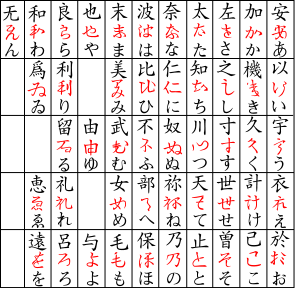
\includegraphics[width=0.9\textwidth]{figs/第01章/第7課:_10majoraspects_fig/Hiragana_Origins.png}

\end{figure}

\begin{figure}[h]
\centering

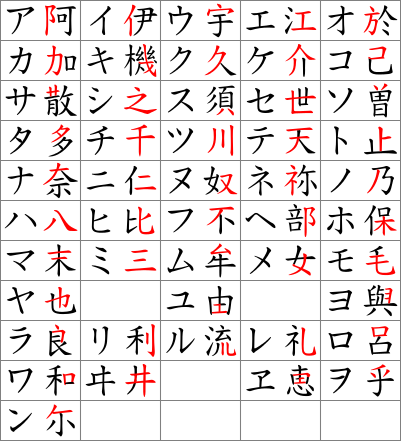
\includegraphics[width=0.9\textwidth]{figs/第01章/第7課:_10majoraspects_fig/Katakana_Origins.png}

\end{figure}

\par{\textbf{History Note }: The first system to be created was \emph{Katakana }カタカナ. It was created thanks to Buddhist monks simplifying the manuscript forms of characters. \emph{Hiragana }ひらがな was created by simplifying the cursive form of characters. \emph{Katakana }カタカナ used to be called "man's hand ( \emph{otokode }男手)" and \emph{Hiragana }ひらがな used to be referred to as "woman's hand ( \emph{on'nade }女手)" as the choice for what script one used was once largely based on one's gender. }

\par{ \emph{Hiragana }ひらがな is seen the most as it is used to spell most words that aren't from foreign languages which \emph{Kanji }漢字 may not be practical or possible. }

\begin{itemize}

\item \textbf{Inflection }- Ex. \emph{Atarashii }新 \textbf{しい }: the part that conjugates is left in \emph{Hiragana }ひらがな. 
\item \textbf{\emph{Kanji }漢字 Replacement }- Ex. \emph{Shiwa }しわ: The symbol 皺 is often deemed too complicated. 
\end{itemize}

\par{\emph{ Katakana }カタカナ is largely used to write foreign loan-words from modern world languages. This includes modern borrowings from Chinese languages. }

\begin{ltabulary}{|P|P|P|P|P|P|}
\hline 

Loan-word & Meaning & Language & Loan-word & Meaning & Language \\ \cline{1-6}

シュウマイ & Barbecued pork & Cantonese & ピザ & Pizza & Italian \\ \cline{1-6}

スポイト & Dropper & Dutch & トナカイ & Reindeer & Ainu \\ \cline{1-6}

\end{ltabulary}

\par{ \emph{Katakana }カタカナ may also be used to write onomatopoeia or used to italicize expressions and even entire sentences. Its purpose for italicization is used heavily in Japanese dictionaries. }

\begin{itemize}

\item \textbf{Italicization }- Ex. \emph{megane }メガネ: Meaning "glasses," this word is typically spelled as 眼鏡. 
\item \textbf{Onomatopoeia }- Ex. \emph{dokan }ドカン (boom). 
\end{itemize}

\par{\textbf{Curriculum Note }: To learn about \emph{Kana }仮名, see also Lessons 3, 4, 355, 356, 357, 364. }

\par{4) English Letters ( \emph{R }\emph{ō }\emph{maji ローマ }字) }

\par{ Though Japanese is largely written with a mix of \emph{Kanji }漢字 and \emph{Kana }仮名, English letters have become incorporated into the spellings of many word, mostly newly coined words. }

\begin{ltabulary}{|P|P|P|P|}
\hline 

 \emph{Piiāru }PR & Public relations &  \emph{Ōeru }OL & Office lady \\ \cline{1-4}

 \emph{Shiidii }CD & CD &  \emph{Diibuidii }DVD & DVD \\ \cline{1-4}

 \emph{Emubui }MV & Music video &  \emph{Tiishatsu }Tシャツ & T-shirt \\ \cline{1-4}

 \emph{Shiiemu }CM & Commercial &  \emph{Piiemu nii ten go }PM2.5 & Particle matter 2.5 \\ \cline{1-4}

 \emph{Eichiaibui }HIV & HIV &  \emph{Erujiibiitii }LGBT & LGBT \\ \cline{1-4}

\end{ltabulary}
\textbf{\hfill\break
Punctuation } Punctuation has largely been borrowed from the Western tradition, but the punctuation marks and rules associated with punctuation have evolved into something quite different. 
\par{ Firstly, there are no spaces between words, and you write to the next line even if this breaks up a word. Text may go down from left to right or down from right to left. Horizontal text was historically right to left. The most basic punctuation marks are shown below. }

\begin{ltabulary}{|P|P|P|P|P|P|P|P|}
\hline 

、 & The comma & 。 & The period & ! & The exclamation mark & ? & The question mark \\ \cline{1-8}

\end{ltabulary}

\par{ Punctuation marks are written with the same space as regular characters. Commas are often where particles are omitted. ! and ? have been borrowed for emphatic purposes to further demonstrate tone and emotion. }

\par{1. ${\overset{\textnormal{わたし}}{\text{私}}}$ は(、)これが ${\overset{\textnormal{す}}{\text{好}}}$ きです。 \hfill\break
\emph{Watashi wa(,) kore ga suki desu. }\hfill\break
I like this. }

\par{2. なに? \hfill\break
\emph{Nani? }\hfill\break
What? }

\par{3. はい! \hfill\break
\emph{Hai! \hfill\break
}Yes!  }

\par{\textbf{Curriculum Note }: To learn more about punctuation, see Lesson 346. }
      
\section{III: Word Order}
 
\begin{center}
\textbf{Basic Word Order } 
\end{center}

\par{ In Japanese, the basic word order is SOV. This stands for subject-object-verb. These terms are defined as follows: }

\begin{itemize}

\item \textbf{Subject }: \emph{The item of discussion in a sentence. }\hfill\break

\item \textbf{Object }: \emph{What an action is directed at. }\hfill\break

\item \textbf{Verb }: \emph{An action or state of being. }
\end{itemize}
 
\par{ Though the basic word order of Japanese involves these parts of a sentence as such, the subject and object may flip positions depending on what is deemed more important to the speaker, and a sentence may be without either or both yet still be grammatical. This means that Japanese exhibits all of the following word orders: SOV, OSV, SV, and OV. Of these,the least frequently used is the OSV word order; however, it is still occasionally used nonetheless. }

\par{ In between the subject and object of a sentence are words called particles. Particles are \textbf{post-positions }that equate to the prepositions of English that indicate the grammatical function(s) of what they follow. }
\hfill\break

\par{\textbf{SOV }\hfill\break
4. クマが ${\overset{\textnormal{さかな}}{\text{魚}}}$ を ${\overset{\textnormal{た}}{\text{食}}}$ べた。 \hfill\break
\emph{Kuma ga sakana wo tabeta. \hfill\break
}The bear ate the fish. }
 
\par{\textbf{OV \hfill\break
}6. ボール + を + ${\overset{\textnormal{な}}{\text{投}}}$ げた。 \hfill\break
\emph{Bōru wo nageta. }\hfill\break
Literally: Ball threw. \hfill\break
Translation: I threw the ball. }
 
\par{\textbf{OSV }\hfill\break
5. ${\overset{\textnormal{さかな}}{\text{魚}}}$ をクマが ${\overset{\textnormal{た}}{\text{食}}}$ べた \hfill\break
\emph{Sakana wo kuma ga tabeta. }\hfill\break
The bear ate the fish. }

\par{\textbf{V }\hfill\break
7. ${\overset{\textnormal{うた}}{\text{歌}}}$ った 。 \hfill\break
\emph{Utatta. \hfill\break
}Literally: Sang. \hfill\break
Translation: I sang.  }

\begin{center}
\textbf{Left-Branching }
\end{center}

\par{ In grammar, "left-branching" refers to modifiers preceding their constituents. For instance, in the English phrase "a tall man," the word "tall" modifies the word "man." This is an example of left-branching in English. However, in English, when a modify becomes too long\slash complex, it goes after its constituent. This is called right-branching. In the examples below, the constituent is in bold while their modifiers are italicized. }

\begin{enumerate}

\item The \emph{kind }\textbf{cat  }(left-branching) 
\item The \emph{smart } \textbf{dog } (left-branching) 
\item The \textbf{cat } \emph{brought back to life } (right-branching) 
\item The \textbf{dog } \emph{chasing its tail } (right-branching) 
\end{enumerate}

\par{ In Japanese, modifiers always go before their constituents no matter how complex they are. }

\par{8. ${\overset{\textnormal{やさ}}{\text{優}}}$ しい ${\overset{\textnormal{ひと}}{\text{人}}}$ \hfill\break
 \emph{Yasashii hito \hfill\break
 }Nice person }

\par{9. ${\overset{\textnormal{がっこう}}{\text{学校}}}$ から ${\overset{\textnormal{かえ}}{\text{帰}}}$ った ${\overset{\textnormal{こども}}{\text{子供}}}$ \hfill\break
 \emph{Gakk }\emph{ō-kara kaetta kodomo \hfill\break
 }Literally: School-from returned kid \hfill\break
Translation: Child who came back from school. }

\begin{center}
\textbf{Typical Structuring of Information }\hfill\break

\end{center}

\par{  In Japanese, word order is not fixated in the way it is in English. Ultimately, the speaker can and normally will organize elements of any given sentence based on what he\slash she deems to be most to least important. However, most sentences are far more predictable than this fluid representation. Typically, information is organized with the following broad ordering. }

\begin{ltabulary}{|P|}
\hline 

TOPIC + TIME + LOCATION + SUBJECT + INDIRECT OBJECT + DIRECT OBJECT + VERB \\

\end{ltabulary}

\par{  The basic word order of SOV is reflected in this ordering, but Japanese typically puts a lot of information before the subject. }

\begin{itemize}

\item The "topic" of a sentence is what the sentence\slash discussion is about. 
\item Time phrases would include expressions such as "today, "tomorrow," etc. 
\item Location phrases would include expressions such as "at Tokyo," "in China," etc. 
\item An \textbf{indirect object }is \emph{a phrase referring to something\slash someone that is a recipient of some action }, but it isn't the primary (direct object). 
\item A \textbf{direct object }is \emph{a phrase that is primarily being affected by the verb }. 
\end{itemize}

\par{10. ${\overset{\textnormal{わたし}}{\text{私}}}$ はきょう、 ${\overset{\textnormal{えき}}{\text{駅}}}$ で ${\overset{\textnormal{ともだち}}{\text{友達}}}$ に ${\overset{\textnormal{ほん}}{\text{本}}}$ をあげました。 \hfill\break
\emph{Watashi-wa ky }\emph{ō, eki-de (ø-ga) to }\emph{modachi-ni hon-wo agemashita. \hfill\break
}Literally: I-as.for, today, station-at (I-subject.marker) friend-to book-object.marker gave. \hfill\break
Trans lation: I gave a book to a friend at the train station today. }

\par{\textbf{Grammar Notes }: \hfill\break
1. Whenever the subject and topic are the same, the subject is not stated but manifests in the grammar as an unspoken zero-pronoun. This rule comes from the general principle of obligatorily omitting syntactically redundant elements, which we'll look at next. \hfill\break
2. The typical ordering of information is almost completely opposite of that of English. }

\par{11. ${\overset{\textnormal{ぞう}}{\text{象}}}$ は ${\overset{\textnormal{はな}}{\text{鼻}}}$ が ${\overset{\textnormal{なが}}{\text{長}}}$ い。 \hfill\break
\emph{Zō-wa hana-ga nagai. }\hfill\break
Literally: Elephants-as.for nose-subject .marker long. \hfill\break
Translation: As for elephants, their noses are long\slash Elephants have long noses. }

\par{\textbf{Grammar Note }: This sentence demonstrates how the subject and topic of a sentence, though related intrinsically with each other, do not have to be the same thing. The pattern shown in this example will be of major focus for us in Lesson 12. }

\par{12. ${\overset{\textnormal{けさじしん}}{\text{今朝地震}}}$ が ${\overset{\textnormal{お}}{\text{起}}}$ きました。 \hfill\break
\emph{Kesa jishin-ga okimashita. }\hfill\break
Literally: This.morning earthquake-subject.marker occurred. \hfill\break
Translation: An earthquake occurred this morning. }

\par{\textbf{Grammar Note }: Not all verbs require objects as demonstrated in Ex. 12. This sentence is perfectly grammatical with just a time phrase, subject, and a verb. }

\par{13. ${\overset{\textnormal{あした}}{\text{明日}}}$ から ${\overset{\textnormal{かれ}}{\text{彼}}}$ に ${\overset{\textnormal{にほんご}}{\text{日本語}}}$ を ${\overset{\textnormal{おし}}{\text{教}}}$ え ${\overset{\textnormal{はじ}}{\text{始}}}$ めます。 \hfill\break
\emph{Ashita-kara kare-ni Nihongo-wo oshiehajimemasu. }\hfill\break
Literally: Tomorrow-from he-to Japanese-direct object. teach.begin. \hfill\break
I will begin teaching Japanese to him as of tomorrow. }

\par{\textbf{Grammar Note }: "To begin teaching" is expressed with a compound verb in Japanese, but the ordering of its components is the opposite of English. In Japanese, the element for "to teach" comes first, and the element for "to begin" is added as a supplementary ending. }

\begin{center}
\textbf{Omission }
\end{center}

\par{ If something is not important at all, it may be omitted altogether, even if it's an element of a sentence that may be grammatically necessary in Japanese. This is evident in how words like "I" and "you," which are a part of an overwhelming of English sentences, are frequently not stated. Of course, the decision between omitting or verbalizing something does imply change in nuance. For now, however, it's important to note that something in an English sentence may not need to transfer over to Japanese. }

\par{14. お ${\overset{\textnormal{なまえ}}{\text{名前}}}$ は ${\overset{\textnormal{なん}}{\text{何}}}$ ですか。 \hfill\break
\emph{O-namae-wa nan desu-ka? }\hfill\break
Literally: Honorific.prefix-name-as.for, name is-question.marker? \hfill\break
Translation: What is your name? }

\par{\textbf{Sentence Note }: There is no word in this example corresponding to "your." }

\par{15. セスと ${\overset{\textnormal{もう}}{\text{申}}}$ します。  \hfill\break
\emph{Sesu-to mōshimasu. }\hfill\break
Literally: Seth-citation.marker called. \hfill\break
Translation: I go by Seth. }

\par{\textbf{Sentence Note }: There is no word in this example corresponding to "I." }

\begin{center}
\textbf{Inversion } 
\end{center}

\par{ It's even possible to mention the verb first and state everything else as an after-statement. This is called inversion. }

\par{16. ${\overset{\textnormal{かな}}{\text{叶}}}$ え、 ${\overset{\textnormal{わたし}}{\text{私}}}$ の ${\overset{\textnormal{ねが}}{\text{願}}}$ いよ。 \hfill\break
\emph{Kanae, watashi-no negai-yo. \hfill\break
}Literally: Come.true I-genitive.marker wish-exclamation.marker \hfill\break
Translation: Come true, oh my wishes.   }

\begin{center}
\textbf{Name Ordering } 
\end{center}

\par{ The hierarchy of information importance also explains why one's family name comes first in Japanese. However, it is important to note that the language actually respects the original ordering of parts of a name if it is from another language. Many learners feel like inverting their name to be more Japanese, but this is not necessary and may end up confusing Japanese people who anticipate the first part of your name to be your given name. }

\begin{ltabulary}{|P|P|P|P|}
\hline 

Barack Obama & バラック・オバマ \hfill\break
\emph{Barakku Obama }& Donald Trump & ドナルド・トランプ \hfill\break
\emph{Donarudo Torampu } \\ \cline{1-4}

Moon Jae-in & ムーン・ジェイン \hfill\break
\emph{M }\emph{ū }\emph{n Je-in } & Kim Jeong Un & 金正恩 \hfill\break
\emph{Kimu Jon Un }\hfill\break
\\ \cline{1-4}

John Smith & ジョン・スミス \hfill\break
Jon Sumisu & Ryo Watanabe & 渡辺亮 \hfill\break
 \emph{Watanabe Ry }\emph{ō }\\ \cline{1-4}

Shinzo Abe & 安倍晋三 \hfill\break
 \emph{Abe Shinzō } & Yu Darvish & ダルビッシュ有 \hfill\break
\emph{Darubisshu Yū }\\ \cline{1-4}

\end{ltabulary}
      
\section{IV: Parts of Speech}
 
\par{ Understanding part of speech ( \emph{hinshi }品詞) is a quintessential to properly harnessing the grammar of a language. As a native speaker of any language, you are privy to instinctively knowing how words relate to one another, how they are similar and dissimilar. Without knowing the names of the categories that exist in your language, you're able to naturally categorize words together in various ways. }

\par{ These categorizations, though, are language specific. Meaning, just because English has words called prepositions, that doesn't mean Japanese does as well. In fact, as we have learned already, prepositions really don't exist in Japanese. Instead, they're replaced by something called particles (post-positions). This, though, is just one instance of how the two languages differ. }

\par{ To begin learning what the parts of speech are in Japanese, it's important to first answer a seemingly simple yet difficult question: what is a word? For English speakers, a word is anything that is written as one unit. In writing, we distinguish words by spaces. However, spacing doesn't always do justice to a word count. Take for instance the following phrases. }

\par{v. Don't (1-2 words) \hfill\break
vi. Music video (1-2 words) }

\par{ The phrase "don't" is a contraction of "do" and "not." Native English speakers typically conceptualize this as one word and do not necessarily deconstruct it in their minds when they use it. Likewise, the phrase "music video" refers specifically to a certain thing that is not solely music nor solely a video. In that sense, you could say it's one word, whereas if you go solely by its spelling you would say that it is two words. Because the word "word" is very vague, for linguistic purposes, the word morpheme is preferred. A morpheme is the smallest unit of meaning that cannot be divided further. This compartmentalization of meaning enables us to properly and objectively study Japanese phrasing for what it is rather than looking at it through an English-stilted mindset. For discussions that follow, depending on how specific things need to be broken up, "word" or "morpheme" will be used. }

\begin{center}
\textbf{Independent VS Ancillary Words }
\end{center}

\par{ There are two kinds of words in Japanese: independent words ( \emph{jiritsugo }自立語) and ancillary words ( \emph{fuzokugo }付属語. Independent words are those that can stand alone. Independent words can further be broken down into conjugatable and non-conjugatable words. Ancillary words, however, cannot stand alone. They too, though, may or may not be conjugatable. }

\par{ In Japanese, there are twelve unique parts of speech that can be classified as either independent or ancillary words. }

\begin{itemize}

\item  Independent Words  ( \emph{Jiritsugo }自立語) \hfill\break
\hfill\break
ー Conjugatable  \hfill\break
\hfill\break
・Verbs ( \emph{Dōshi }動詞)\dothyp{}\dothyp{}\dothyp{}\dothyp{}\dothyp{}\dothyp{}\dothyp{}\dothyp{}\dothyp{}\dothyp{}\dothyp{}\dothyp{}\dothyp{}\dothyp{}\dothyp{}\dothyp{}\dothyp{}\dothyp{}\dothyp{}\dothyp{}\dothyp{}\dothyp{}\dothyp{}\dothyp{}\dothyp{}\dothyp{}\dothyp{}\dothyp{}\dothyp{}\dothyp{}\dothyp{}\dothyp{}\dothyp{}\dothyp{}\dothyp{}\dothyp{}\dothyp{}\dothyp{}\dothyp{}\dothyp{}\dothyp{}\dothyp{}\dothyp{}\dothyp{}\dothyp{}\dothyp{}\dothyp{}\dothyp{}..Lessons 16, 17, 18, etc. \hfill\break
  \emph{A \textbf{verb }is a word that describes an action, state, or occurrence. } \hfill\break
・Adjectives ( \emph{Keiyōshi }形容詞) \dothyp{}\dothyp{}\dothyp{}\dothyp{}\dothyp{}\dothyp{}\dothyp{}\dothyp{}\dothyp{}\dothyp{}\dothyp{}\dothyp{}\dothyp{}\dothyp{}\dothyp{}\dothyp{}\dothyp{}\dothyp{}\dothyp{}\dothyp{}\dothyp{}\dothyp{}\dothyp{}\dothyp{}\dothyp{}\dothyp{}\dothyp{}\dothyp{}\dothyp{}\dothyp{}\dothyp{}\dothyp{}\dothyp{}.Lessons 13, 50, 52 \hfill\break
 \emph{An \textbf{adjective }is a word that describes an attribute. }\hfill\break
・Adjectival Nouns ( \emph{Keiyōdōshi }形容動詞) \dothyp{}\dothyp{}\dothyp{}\dothyp{}\dothyp{}\dothyp{}\dothyp{}\dothyp{}\dothyp{}\dothyp{}\dothyp{}\dothyp{}\dothyp{}\dothyp{}\dothyp{}.Lessons 14, 51, 53, etc. \hfill\break
  \emph{An \textbf{adjectival noun }is a word that describes an attribute while also being noun-like. \hfill\break
}\hfill\break
ー Not Conjugatable  \hfill\break
\hfill\break
・Nouns ( \emph{Meishi }名詞)\dothyp{}\dothyp{}\dothyp{}\dothyp{}\dothyp{}\dothyp{}\dothyp{}\dothyp{}\dothyp{}\dothyp{}\dothyp{}\dothyp{}\dothyp{}\dothyp{}\dothyp{}\dothyp{}\dothyp{}\dothyp{}\dothyp{}\dothyp{}\dothyp{}\dothyp{}\dothyp{}\dothyp{}\dothyp{}\dothyp{}\dothyp{}\dothyp{}\dothyp{}\dothyp{}\dothyp{}\dothyp{}\dothyp{}\dothyp{}\dothyp{}\dothyp{}\dothyp{}\dothyp{}\dothyp{}\dothyp{}\dothyp{}\dothyp{}\dothyp{}\dothyp{}\dothyp{}\dothyp{}\dothyp{}\dothyp{}Lesson 8 \hfill\break
  \emph{A \textbf{noun }is a word that describes a person, place, state, quality, event, or thing. }\hfill\break
・Pronouns ( \emph{Daimeishi }代名詞)\dothyp{}\dothyp{}\dothyp{}\dothyp{}\dothyp{}\dothyp{}\dothyp{}\dothyp{}\dothyp{}\dothyp{}\dothyp{}\dothyp{}\dothyp{}\dothyp{}\dothyp{}\dothyp{}\dothyp{}\dothyp{}\dothyp{}\dothyp{}\dothyp{}\dothyp{}\dothyp{}\dothyp{}\dothyp{}\dothyp{}\dothyp{}\dothyp{}\dothyp{}\dothyp{}\dothyp{}\dothyp{}\dothyp{}.Lessons 8, 84, 191 \hfill\break
  \emph{A \textbf{pronoun }is a word that indirectly describes a person, direction, or thing.  }\hfill\break
・Numbers ( \emph{Sūshi }数詞)\dothyp{}\dothyp{}\dothyp{}\dothyp{}\dothyp{}\dothyp{}\dothyp{}\dothyp{}\dothyp{}\dothyp{}\dothyp{}\dothyp{}\dothyp{}\dothyp{}\dothyp{}\dothyp{}\dothyp{}\dothyp{}\dothyp{}\dothyp{}\dothyp{}\dothyp{}\dothyp{}\dothyp{}\dothyp{}\dothyp{}\dothyp{}\dothyp{}\dothyp{}\dothyp{}\dothyp{}\dothyp{}\dothyp{}\dothyp{}\dothyp{}\dothyp{}\dothyp{}\dothyp{}\dothyp{}\dothyp{}\dothyp{}\dothyp{}\dothyp{}\dothyp{}\dothyp{}Lessons 27, 28, 29, 193, etc. \hfill\break
 \emph{A \textbf{number }is a word that counts or measures entities. }\hfill\break
・Adnominal Adjectives ( \emph{Rentaishi }連体詞)\dothyp{}\dothyp{}\dothyp{}\dothyp{}\dothyp{}\dothyp{}\dothyp{}\dothyp{}\dothyp{}\dothyp{}\dothyp{}\dothyp{}\dothyp{}\dothyp{}\dothyp{}Lessons 60 \& 303 \hfill\break
  \emph{An \textbf{adnominal adjective }is a word that describes an attribute by directly modifying a noun. }\hfill\break
 ・Adverbs ( \emph{Fukushi }副詞)\dothyp{}\dothyp{}\dothyp{}\dothyp{}\dothyp{}\dothyp{}\dothyp{}\dothyp{}\dothyp{}\dothyp{}\dothyp{}\dothyp{}\dothyp{}\dothyp{}\dothyp{}\dothyp{}\dothyp{}\dothyp{}\dothyp{}\dothyp{}\dothyp{}\dothyp{}\dothyp{}\dothyp{}\dothyp{}\dothyp{}\dothyp{}\dothyp{}\dothyp{}\dothyp{}\dothyp{}\dothyp{}\dothyp{}\dothyp{}\dothyp{}\dothyp{}\dothyp{}\dothyp{}\dothyp{}\dothyp{}\dothyp{}\dothyp{}Lessons 48, 49, 154, 293, etc. \hfill\break
  \emph{An \textbf{adverb }is a word that qualifies an adjective, adjectival noun, or a verb. }\hfill\break
・Conjunctions ( \emph{Setsuzokushi }接続詞)\dothyp{}\dothyp{}\dothyp{}\dothyp{}\dothyp{}\dothyp{}\dothyp{}\dothyp{}\dothyp{}\dothyp{}\dothyp{}\dothyp{}\dothyp{}\dothyp{}\dothyp{}\dothyp{}\dothyp{}\dothyp{}\dothyp{}\dothyp{}\dothyp{}.Lesson 169 \hfill\break
  \emph{A }\textbf{conjunction }\emph{is a word that connects sentence together. }\hfill\break
・Interjections ( \emph{Kandōshi }感動詞)\dothyp{}\dothyp{}\dothyp{}\dothyp{}\dothyp{}\dothyp{}\dothyp{}\dothyp{}\dothyp{}\dothyp{}\dothyp{}\dothyp{}\dothyp{}\dothyp{}\dothyp{}\dothyp{}\dothyp{}\dothyp{}\dothyp{}\dothyp{}\dothyp{}\dothyp{}\dothyp{}\dothyp{}\dothyp{}\dothyp{}\dothyp{}..Lesson 200 \hfill\break
 \emph{An \textbf{interjection }is a word that represents an abrupt remark. \hfill\break
\hfill\break
}
\item Ancillary Words  ( \emph{Fuzokugo }付属語) \hfill\break
\hfill\break
ー Conjugatable \hfill\break
\hfill\break
・Auxiliary Verbs ( \emph{Jodōshi }助動詞)\dothyp{}\dothyp{}\dothyp{}\dothyp{}\dothyp{}\dothyp{}\dothyp{}\dothyp{}\dothyp{}\dothyp{}\dothyp{}\dothyp{}\dothyp{}\dothyp{}\dothyp{}\dothyp{}\dothyp{}\dothyp{}\dothyp{}\dothyp{}\dothyp{}\dothyp{}\dothyp{}\dothyp{}\dothyp{}\dothyp{}\dothyp{}Lessons 9, 10, 36, 37, etc. \hfill\break
 \emph{An \textbf{auxiliary verb }is an ending that attaches to a conjugatable part of speech. }\hfill\break
\hfill\break
ー Not Conjugatable \hfill\break
\hfill\break
・Particles ( \emph{Joshi }助詞)\dothyp{}\dothyp{}\dothyp{}\dothyp{}\dothyp{}\dothyp{}\dothyp{}\dothyp{}\dothyp{}\dothyp{}\dothyp{}\dothyp{}\dothyp{}\dothyp{}\dothyp{}\dothyp{}\dothyp{}\dothyp{}\dothyp{}\dothyp{}\dothyp{}\dothyp{}\dothyp{}\dothyp{}\dothyp{}\dothyp{}\dothyp{}\dothyp{}\dothyp{}\dothyp{}\dothyp{}\dothyp{}\dothyp{}\dothyp{}\dothyp{}\dothyp{}\dothyp{}\dothyp{}\dothyp{}\dothyp{}\dothyp{}\dothyp{}..Lessons 11, 12, 15, 19, 20, etc. \hfill\break
 \emph{A \textbf{particle }is a word that follows what it modifies to indicate its function. }
\end{itemize}

\begin{center}
\textbf{The Six Kinds of Particles } 
\end{center}

\par{ Particles arguably constitute the most difficult part of speech to master. This is because there are many grammatical functions a phrase can have in a sentence, and the grammatical functions that Japanese chooses to make evident may not always be those that are of grammatical importance in English. }

\par{ Of all the possible functions and\slash or purposes a particle could possibly express, they are all manifested in only a finite number of particles that far outnumber the roles they have. Similarly to how prepositions overlap in English, many particles at times behave similarly to others. Although it will take time to truly master the various particles of Japanese, a considerable amount of heartache can be avoided by knowing what to expect. }

\par{ There are six main types of particles: case, parallel, conjunctive, final, adverbial, and bound. Particles may be categorized differently depending on how they're used. Below you will find these categories defined with many examples of each. Note that the lists are not necessarily exhaustive. }

\begin{itemize}

\item \textbf{Case Particle ( \emph{Kaku joshi }格助詞) }: A particle that indicates the grammatical function of a word in a sentence. Some are prone to being omitted if their functions are deemed unnecessary to make explicitly clear. \hfill\break
 \hfill\break
ー \emph{Ga }が\dothyp{}\dothyp{}\dothyp{}\dothyp{}\dothyp{}\dothyp{}\dothyp{}\dothyp{}\dothyp{}\dothyp{}\dothyp{}\dothyp{}\dothyp{}\dothyp{}\dothyp{}\dothyp{}\dothyp{}\dothyp{}\dothyp{}\dothyp{}\dothyp{}\dothyp{}\dothyp{}\dothyp{}\dothyp{}\dothyp{}\dothyp{}\dothyp{}\dothyp{}\dothyp{}\dothyp{}\dothyp{}\dothyp{}\dothyp{}\dothyp{}\dothyp{}.Lesson 11, 167 \hfill\break
ー \emph{Wo }を\dothyp{}\dothyp{}\dothyp{}\dothyp{}\dothyp{}\dothyp{}\dothyp{}\dothyp{}\dothyp{}\dothyp{}\dothyp{}\dothyp{}\dothyp{}\dothyp{}\dothyp{}\dothyp{}\dothyp{}\dothyp{}\dothyp{}\dothyp{}\dothyp{}\dothyp{}\dothyp{}\dothyp{}\dothyp{}\dothyp{}\dothyp{}\dothyp{}\dothyp{}\dothyp{}\dothyp{}\dothyp{}\dothyp{}\dothyp{}\dothyp{}\dothyp{}.Lesson 15, 167, 183 \hfill\break
ー \emph{Ni }に\dothyp{}\dothyp{}\dothyp{}\dothyp{}\dothyp{}\dothyp{}\dothyp{}\dothyp{}\dothyp{}\dothyp{}\dothyp{}\dothyp{}\dothyp{}\dothyp{}\dothyp{}\dothyp{}\dothyp{}\dothyp{}\dothyp{}\dothyp{}\dothyp{}\dothyp{}\dothyp{}\dothyp{}\dothyp{}\dothyp{}\dothyp{}\dothyp{}\dothyp{}\dothyp{}\dothyp{}\dothyp{}\dothyp{}\dothyp{}\dothyp{}\dothyp{}\dothyp{}\dothyp{}\dothyp{}Lessons 31, 41, 66, 117 \hfill\break
― \emph{No }の\dothyp{}\dothyp{}\dothyp{}\dothyp{}\dothyp{}\dothyp{}\dothyp{}\dothyp{}\dothyp{}\dothyp{}\dothyp{}\dothyp{}\dothyp{}\dothyp{}\dothyp{}\dothyp{}\dothyp{}\dothyp{}\dothyp{}\dothyp{}\dothyp{}\dothyp{}\dothyp{}\dothyp{}\dothyp{}\dothyp{}\dothyp{}\dothyp{}\dothyp{}\dothyp{}\dothyp{}\dothyp{}\dothyp{}\dothyp{}\dothyp{}\dothyp{}..Lesson 89 \hfill\break
― \emph{E }へ\dothyp{}\dothyp{}\dothyp{}\dothyp{}\dothyp{}\dothyp{}\dothyp{}\dothyp{}\dothyp{}\dothyp{}\dothyp{}\dothyp{}\dothyp{}\dothyp{}\dothyp{}\dothyp{}\dothyp{}\dothyp{}\dothyp{}\dothyp{}\dothyp{}\dothyp{}\dothyp{}\dothyp{}\dothyp{}\dothyp{}\dothyp{}\dothyp{}\dothyp{}\dothyp{}\dothyp{}\dothyp{}\dothyp{}\dothyp{}\dothyp{}\dothyp{}\dothyp{}\dothyp{}\dothyp{}.Lesson 32 \hfill\break
ー \emph{De }で\dothyp{}\dothyp{}\dothyp{}\dothyp{}\dothyp{}\dothyp{}\dothyp{}\dothyp{}\dothyp{}\dothyp{}\dothyp{}\dothyp{}\dothyp{}\dothyp{}\dothyp{}\dothyp{}\dothyp{}\dothyp{}\dothyp{}\dothyp{}\dothyp{}\dothyp{}\dothyp{}\dothyp{}\dothyp{}\dothyp{}\dothyp{}\dothyp{}\dothyp{}\dothyp{}\dothyp{}\dothyp{}\dothyp{}\dothyp{}\dothyp{}\dothyp{}..Lessons 33, 90 \hfill\break
ー \emph{To }と\dothyp{}\dothyp{}\dothyp{}\dothyp{}\dothyp{}\dothyp{}\dothyp{}\dothyp{}\dothyp{}\dothyp{}\dothyp{}\dothyp{}\dothyp{}\dothyp{}\dothyp{}\dothyp{}\dothyp{}\dothyp{}\dothyp{}\dothyp{}\dothyp{}\dothyp{}\dothyp{}\dothyp{}\dothyp{}\dothyp{}\dothyp{}\dothyp{}\dothyp{}\dothyp{}\dothyp{}\dothyp{}\dothyp{}\dothyp{}\dothyp{}\dothyp{}\dothyp{}\dothyp{}\dothyp{}Lesson 66 \hfill\break
ー \emph{Kara }から\dothyp{}\dothyp{}\dothyp{}\dothyp{}\dothyp{}\dothyp{}\dothyp{}\dothyp{}\dothyp{}\dothyp{}\dothyp{}\dothyp{}\dothyp{}\dothyp{}\dothyp{}\dothyp{}\dothyp{}\dothyp{}\dothyp{}\dothyp{}\dothyp{}\dothyp{}\dothyp{}\dothyp{}\dothyp{}\dothyp{}\dothyp{}\dothyp{}\dothyp{}\dothyp{}..Lessons 46, 117, 256 \hfill\break
ー \emph{Yori }より\dothyp{}\dothyp{}\dothyp{}\dothyp{}\dothyp{}\dothyp{}\dothyp{}\dothyp{}\dothyp{}\dothyp{}\dothyp{}\dothyp{}\dothyp{}\dothyp{}\dothyp{}\dothyp{}\dothyp{}\dothyp{}\dothyp{}\dothyp{}\dothyp{}\dothyp{}\dothyp{}\dothyp{}\dothyp{}\dothyp{}\dothyp{}\dothyp{}\dothyp{}\dothyp{}\dothyp{}\dothyp{}\dothyp{}Lesson 144 \hfill\break
\hfill\break

\item \textbf{Parallel Particle ( \emph{Heiritsu joshi }並立助詞) }: A particle that juxtaposes two or more things together. \hfill\break
\hfill\break
ー \emph{To }と\dothyp{}\dothyp{}\dothyp{}\dothyp{}\dothyp{}\dothyp{}\dothyp{}\dothyp{}\dothyp{}\dothyp{}\dothyp{}\dothyp{}\dothyp{}\dothyp{}\dothyp{}\dothyp{}\dothyp{}\dothyp{}\dothyp{}\dothyp{}\dothyp{}\dothyp{}\dothyp{}\dothyp{}\dothyp{}\dothyp{}\dothyp{}\dothyp{}\dothyp{}\dothyp{}\dothyp{}\dothyp{}\dothyp{}\dothyp{}\dothyp{}\dothyp{}\dothyp{}\dothyp{}\dothyp{}Lesson 40 \hfill\break
ー \emph{No }の\dothyp{}\dothyp{}\dothyp{}\dothyp{}\dothyp{}\dothyp{}\dothyp{}\dothyp{}\dothyp{}\dothyp{}\dothyp{}\dothyp{}\dothyp{}\dothyp{}\dothyp{}\dothyp{}\dothyp{}\dothyp{}\dothyp{}\dothyp{}\dothyp{}\dothyp{}\dothyp{}\dothyp{}\dothyp{}\dothyp{}\dothyp{}\dothyp{}\dothyp{}\dothyp{}\dothyp{}\dothyp{}\dothyp{}\dothyp{}\dothyp{}\dothyp{}..Lesson 30 \hfill\break
ー \emph{Ni }に\dothyp{}\dothyp{}\dothyp{}\dothyp{}\dothyp{}\dothyp{}\dothyp{}\dothyp{}\dothyp{}\dothyp{}\dothyp{}\dothyp{}\dothyp{}\dothyp{}\dothyp{}\dothyp{}\dothyp{}\dothyp{}\dothyp{}\dothyp{}\dothyp{}\dothyp{}\dothyp{}\dothyp{}\dothyp{}\dothyp{}\dothyp{}\dothyp{}\dothyp{}\dothyp{}\dothyp{}\dothyp{}\dothyp{}\dothyp{}\dothyp{}\dothyp{}\dothyp{}\dothyp{}\dothyp{}Lesson 41 \hfill\break
ー \emph{Ya }や\dothyp{}\dothyp{}\dothyp{}\dothyp{}\dothyp{}\dothyp{}\dothyp{}\dothyp{}\dothyp{}\dothyp{}\dothyp{}\dothyp{}\dothyp{}\dothyp{}\dothyp{}\dothyp{}\dothyp{}\dothyp{}\dothyp{}\dothyp{}\dothyp{}\dothyp{}\dothyp{}\dothyp{}\dothyp{}\dothyp{}\dothyp{}\dothyp{}\dothyp{}\dothyp{}\dothyp{}\dothyp{}\dothyp{}\dothyp{}\dothyp{}\dothyp{}..Lesson 68 \hfill\break
ー \emph{Yara }やら\dothyp{}\dothyp{}\dothyp{}\dothyp{}\dothyp{}\dothyp{}\dothyp{}\dothyp{}\dothyp{}\dothyp{}\dothyp{}\dothyp{}\dothyp{}\dothyp{}\dothyp{}\dothyp{}\dothyp{}\dothyp{}\dothyp{}\dothyp{}\dothyp{}\dothyp{}\dothyp{}\dothyp{}\dothyp{}\dothyp{}\dothyp{}\dothyp{}\dothyp{}\dothyp{}.Lesson 302 \hfill\break
ー \emph{Ka }か\dothyp{}\dothyp{}\dothyp{}\dothyp{}\dothyp{}\dothyp{}\dothyp{}\dothyp{}\dothyp{}\dothyp{}\dothyp{}\dothyp{}\dothyp{}\dothyp{}\dothyp{}\dothyp{}\dothyp{}\dothyp{}\dothyp{}\dothyp{}\dothyp{}\dothyp{}\dothyp{}\dothyp{}\dothyp{}\dothyp{}\dothyp{}\dothyp{}\dothyp{}\dothyp{}\dothyp{}\dothyp{}\dothyp{}\dothyp{}\dothyp{}\dothyp{}..Lesson 164 \hfill\break
ー \emph{Nari }なり\dothyp{}\dothyp{}\dothyp{}\dothyp{}\dothyp{}\dothyp{}\dothyp{}\dothyp{}\dothyp{}\dothyp{}\dothyp{}\dothyp{}\dothyp{}\dothyp{}\dothyp{}\dothyp{}\dothyp{}\dothyp{}\dothyp{}\dothyp{}\dothyp{}\dothyp{}\dothyp{}\dothyp{}\dothyp{}\dothyp{}\dothyp{}\dothyp{}\dothyp{}\dothyp{}..Lesson 302 \hfill\break
ー \emph{Dano }だの\dothyp{}\dothyp{}\dothyp{}\dothyp{}\dothyp{}\dothyp{}\dothyp{}\dothyp{}\dothyp{}\dothyp{}\dothyp{}\dothyp{}\dothyp{}\dothyp{}\dothyp{}\dothyp{}\dothyp{}\dothyp{}\dothyp{}\dothyp{}\dothyp{}\dothyp{}\dothyp{}\dothyp{}\dothyp{}\dothyp{}\dothyp{}\dothyp{}\dothyp{}\dothyp{}Lesson 304 \hfill\break
― \emph{Toka }とか\dothyp{}\dothyp{}\dothyp{}\dothyp{}\dothyp{}\dothyp{}\dothyp{}\dothyp{}\dothyp{}\dothyp{}\dothyp{}\dothyp{}\dothyp{}\dothyp{}\dothyp{}\dothyp{}\dothyp{}\dothyp{}\dothyp{}\dothyp{}\dothyp{}\dothyp{}\dothyp{}\dothyp{}\dothyp{}\dothyp{}\dothyp{}\dothyp{}\dothyp{}\dothyp{}.Lesson 141 \hfill\break
\hfill\break

\item \textbf{Conjunctive Particle ( \emph{Setsuzoku joshi }接続助詞) }: A particle that connects clauses (parts of a sentence) together. \hfill\break
\hfill\break
ー \emph{Ga }が\dothyp{}\dothyp{}\dothyp{}\dothyp{}\dothyp{}\dothyp{}\dothyp{}\dothyp{}\dothyp{}\dothyp{}\dothyp{}\dothyp{}\dothyp{}\dothyp{}\dothyp{}\dothyp{}\dothyp{}\dothyp{}\dothyp{}\dothyp{}\dothyp{}\dothyp{}\dothyp{}\dothyp{}\dothyp{}\dothyp{}\dothyp{}\dothyp{}\dothyp{}\dothyp{}\dothyp{}\dothyp{}\dothyp{}\dothyp{}\dothyp{}\dothyp{}.Lesson 76 \hfill\break
ー \emph{Ke(re)do }け(れ)ど\dothyp{}\dothyp{}\dothyp{}\dothyp{}\dothyp{}\dothyp{}\dothyp{}\dothyp{}\dothyp{}\dothyp{}\dothyp{}\dothyp{}.Lesson 76 \hfill\break
ー \emph{Ba }ば\dothyp{}\dothyp{}\dothyp{}\dothyp{}\dothyp{}\dothyp{}\dothyp{}\dothyp{}\dothyp{}\dothyp{}\dothyp{}\dothyp{}\dothyp{}\dothyp{}\dothyp{}\dothyp{}\dothyp{}\dothyp{}\dothyp{}\dothyp{}\dothyp{}\dothyp{}\dothyp{}\dothyp{}\dothyp{}\dothyp{}\dothyp{}\dothyp{}\dothyp{}\dothyp{}\dothyp{}\dothyp{}\dothyp{}\dothyp{}\dothyp{}\dothyp{}.Lessons 109, 110, 111 \hfill\break
ー \emph{To }と\dothyp{}\dothyp{}\dothyp{}\dothyp{}\dothyp{}\dothyp{}\dothyp{}\dothyp{}\dothyp{}\dothyp{}\dothyp{}\dothyp{}\dothyp{}\dothyp{}\dothyp{}\dothyp{}\dothyp{}\dothyp{}\dothyp{}\dothyp{}\dothyp{}\dothyp{}\dothyp{}\dothyp{}\dothyp{}\dothyp{}\dothyp{}\dothyp{}\dothyp{}\dothyp{}\dothyp{}\dothyp{}\dothyp{}\dothyp{}\dothyp{}\dothyp{}.Lessons 109, 110, 111 \hfill\break
― \emph{Tara }たら\dothyp{}\dothyp{}\dothyp{}\dothyp{}\dothyp{}\dothyp{}\dothyp{}\dothyp{}\dothyp{}\dothyp{}\dothyp{}\dothyp{}\dothyp{}\dothyp{}\dothyp{}\dothyp{}\dothyp{}\dothyp{}\dothyp{}\dothyp{}\dothyp{}\dothyp{}\dothyp{}\dothyp{}\dothyp{}\dothyp{}\dothyp{}\dothyp{}\dothyp{}\dothyp{}Lessons 109, 110, 111 \hfill\break
ー \emph{Temo }ても\dothyp{}\dothyp{}\dothyp{}\dothyp{}\dothyp{}\dothyp{}\dothyp{}\dothyp{}\dothyp{}\dothyp{}\dothyp{}\dothyp{}\dothyp{}\dothyp{}\dothyp{}\dothyp{}\dothyp{}\dothyp{}\dothyp{}\dothyp{}\dothyp{}\dothyp{}\dothyp{}\dothyp{}\dothyp{}\dothyp{}\dothyp{}.Lesson 67 \hfill\break
ー \emph{Node }ので\dothyp{}\dothyp{}\dothyp{}\dothyp{}\dothyp{}\dothyp{}\dothyp{}\dothyp{}\dothyp{}\dothyp{}\dothyp{}\dothyp{}\dothyp{}\dothyp{}\dothyp{}\dothyp{}\dothyp{}\dothyp{}\dothyp{}\dothyp{}\dothyp{}\dothyp{}\dothyp{}\dothyp{}\dothyp{}\dothyp{}\dothyp{}.Lesson 57 \hfill\break
ー \emph{Noni }のに\dothyp{}\dothyp{}\dothyp{}\dothyp{}\dothyp{}\dothyp{}\dothyp{}\dothyp{}\dothyp{}\dothyp{}\dothyp{}\dothyp{}\dothyp{}\dothyp{}\dothyp{}\dothyp{}\dothyp{}\dothyp{}\dothyp{}\dothyp{}\dothyp{}\dothyp{}\dothyp{}\dothyp{}\dothyp{}\dothyp{}\dothyp{}..Lesson 58 \hfill\break
ー \emph{Kara }から\dothyp{}\dothyp{}\dothyp{}\dothyp{}\dothyp{}\dothyp{}\dothyp{}\dothyp{}\dothyp{}\dothyp{}\dothyp{}\dothyp{}\dothyp{}\dothyp{}\dothyp{}\dothyp{}\dothyp{}\dothyp{}\dothyp{}\dothyp{}\dothyp{}\dothyp{}\dothyp{}\dothyp{}\dothyp{}\dothyp{}\dothyp{}..Lesson 57 \hfill\break
ー \emph{Shi }し\dothyp{}\dothyp{}\dothyp{}\dothyp{}\dothyp{}\dothyp{}\dothyp{}\dothyp{}\dothyp{}\dothyp{}\dothyp{}\dothyp{}\dothyp{}\dothyp{}\dothyp{}\dothyp{}\dothyp{}\dothyp{}\dothyp{}\dothyp{}\dothyp{}\dothyp{}\dothyp{}\dothyp{}\dothyp{}\dothyp{}\dothyp{}\dothyp{}\dothyp{}\dothyp{}\dothyp{}\dothyp{}\dothyp{}..Lesson 69 \hfill\break
ー \emph{Te }て\dothyp{}\dothyp{}\dothyp{}\dothyp{}\dothyp{}\dothyp{}\dothyp{}\dothyp{}\dothyp{}\dothyp{}\dothyp{}\dothyp{}\dothyp{}\dothyp{}\dothyp{}\dothyp{}\dothyp{}\dothyp{}\dothyp{}\dothyp{}\dothyp{}\dothyp{}\dothyp{}\dothyp{}\dothyp{}\dothyp{}\dothyp{}\dothyp{}\dothyp{}\dothyp{}\dothyp{}\dothyp{}\dothyp{}\dothyp{}\dothyp{}\dothyp{}Lesson 26 \hfill\break
ー \emph{Nagara }ながら\dothyp{}\dothyp{}\dothyp{}\dothyp{}\dothyp{}\dothyp{}\dothyp{}\dothyp{}\dothyp{}\dothyp{}\dothyp{}\dothyp{}\dothyp{}\dothyp{}\dothyp{}\dothyp{}\dothyp{}\dothyp{}\dothyp{}\dothyp{}\dothyp{}Lessons 104, 288 \hfill\break
ー \emph{Tsutsu }つつ\dothyp{}\dothyp{}\dothyp{}\dothyp{}\dothyp{}\dothyp{}\dothyp{}\dothyp{}\dothyp{}\dothyp{}\dothyp{}\dothyp{}\dothyp{}\dothyp{}\dothyp{}\dothyp{}\dothyp{}\dothyp{}\dothyp{}\dothyp{}\dothyp{}\dothyp{}\dothyp{}\dothyp{}..Lesson 289 \hfill\break
ー \emph{Tari }たり\dothyp{}\dothyp{}\dothyp{}\dothyp{}\dothyp{}\dothyp{}\dothyp{}\dothyp{}\dothyp{}\dothyp{}\dothyp{}\dothyp{}\dothyp{}\dothyp{}\dothyp{}\dothyp{}\dothyp{}\dothyp{}\dothyp{}\dothyp{}\dothyp{}\dothyp{}\dothyp{}\dothyp{}\dothyp{}\dothyp{}\dothyp{}\dothyp{}\dothyp{}\dothyp{}.Lesson 101 \hfill\break
― \emph{Domo }ども\dothyp{}\dothyp{}\dothyp{}\dothyp{}\dothyp{}\dothyp{}\dothyp{}\dothyp{}\dothyp{}\dothyp{}\dothyp{}\dothyp{}\dothyp{}\dothyp{}\dothyp{}\dothyp{}\dothyp{}\dothyp{}\dothyp{}\dothyp{}\dothyp{}\dothyp{}\dothyp{}\dothyp{}\dothyp{}\dothyp{}\dothyp{}Lesson 304 \hfill\break
\hfill\break

\item \textbf{Final Particle ( \emph{Shū-joshi }終助詞) }: A particle placed at the end of a phrase to provide emotional context. \hfill\break
\hfill\break
― \emph{Ka }か\dothyp{}\dothyp{}\dothyp{}\dothyp{}\dothyp{}\dothyp{}\dothyp{}\dothyp{}\dothyp{}\dothyp{}\dothyp{}\dothyp{}\dothyp{}\dothyp{}\dothyp{}\dothyp{}\dothyp{}\dothyp{}\dothyp{}\dothyp{}\dothyp{}\dothyp{}\dothyp{}\dothyp{}\dothyp{}\dothyp{}\dothyp{}\dothyp{}\dothyp{}\dothyp{}\dothyp{}\dothyp{}\dothyp{}\dothyp{}\dothyp{}\dothyp{}Lessons 19, 20 \hfill\break
ー \emph{Yo }よ\dothyp{}\dothyp{}\dothyp{}\dothyp{}\dothyp{}\dothyp{}\dothyp{}\dothyp{}\dothyp{}\dothyp{}\dothyp{}\dothyp{}\dothyp{}\dothyp{}\dothyp{}\dothyp{}\dothyp{}\dothyp{}\dothyp{}\dothyp{}\dothyp{}\dothyp{}\dothyp{}\dothyp{}\dothyp{}\dothyp{}\dothyp{}\dothyp{}\dothyp{}\dothyp{}\dothyp{}\dothyp{}\dothyp{}\dothyp{}\dothyp{}\dothyp{}Lesson 77 \hfill\break
ー \emph{Ne }ね\dothyp{}\dothyp{}\dothyp{}\dothyp{}\dothyp{}\dothyp{}\dothyp{}\dothyp{}\dothyp{}\dothyp{}\dothyp{}\dothyp{}\dothyp{}\dothyp{}\dothyp{}\dothyp{}\dothyp{}\dothyp{}\dothyp{}\dothyp{}\dothyp{}\dothyp{}\dothyp{}\dothyp{}\dothyp{}\dothyp{}\dothyp{}\dothyp{}\dothyp{}\dothyp{}\dothyp{}\dothyp{}\dothyp{}\dothyp{}\dothyp{}\dothyp{}Lesson 77 \hfill\break
ー \emph{Wa }わ\dothyp{}\dothyp{}\dothyp{}\dothyp{}\dothyp{}\dothyp{}\dothyp{}\dothyp{}\dothyp{}\dothyp{}\dothyp{}\dothyp{}\dothyp{}\dothyp{}\dothyp{}\dothyp{}\dothyp{}\dothyp{}\dothyp{}\dothyp{}\dothyp{}\dothyp{}\dothyp{}\dothyp{}\dothyp{}\dothyp{}\dothyp{}\dothyp{}\dothyp{}\dothyp{}\dothyp{}\dothyp{}\dothyp{}..Lesson 78 \hfill\break
― \emph{Te }て\dothyp{}\dothyp{}\dothyp{}\dothyp{}\dothyp{}\dothyp{}\dothyp{}\dothyp{}\dothyp{}\dothyp{}\dothyp{}\dothyp{}\dothyp{}\dothyp{}\dothyp{}\dothyp{}\dothyp{}\dothyp{}\dothyp{}\dothyp{}\dothyp{}\dothyp{}\dothyp{}\dothyp{}\dothyp{}\dothyp{}\dothyp{}\dothyp{}\dothyp{}\dothyp{}\dothyp{}\dothyp{}\dothyp{}\dothyp{}\dothyp{}\dothyp{}Lesson 30 \hfill\break
ー \emph{Na }な\dothyp{}\dothyp{}\dothyp{}\dothyp{}\dothyp{}\dothyp{}\dothyp{}\dothyp{}\dothyp{}\dothyp{}\dothyp{}\dothyp{}\dothyp{}\dothyp{}\dothyp{}\dothyp{}\dothyp{}\dothyp{}\dothyp{}\dothyp{}\dothyp{}\dothyp{}\dothyp{}\dothyp{}\dothyp{}\dothyp{}\dothyp{}\dothyp{}\dothyp{}\dothyp{}\dothyp{}\dothyp{}\dothyp{}..Lesson 78 \hfill\break
ー \emph{Zo }ぞ\dothyp{}\dothyp{}\dothyp{}\dothyp{}\dothyp{}\dothyp{}\dothyp{}\dothyp{}\dothyp{}\dothyp{}\dothyp{}\dothyp{}\dothyp{}\dothyp{}\dothyp{}\dothyp{}\dothyp{}\dothyp{}\dothyp{}\dothyp{}\dothyp{}\dothyp{}\dothyp{}\dothyp{}\dothyp{}\dothyp{}\dothyp{}\dothyp{}\dothyp{}\dothyp{}\dothyp{}\dothyp{}\dothyp{}..Lesson 78 \hfill\break
ー \emph{Ze }ぜ\dothyp{}\dothyp{}\dothyp{}\dothyp{}\dothyp{}\dothyp{}\dothyp{}\dothyp{}\dothyp{}\dothyp{}\dothyp{}\dothyp{}\dothyp{}\dothyp{}\dothyp{}\dothyp{}\dothyp{}\dothyp{}\dothyp{}\dothyp{}\dothyp{}\dothyp{}\dothyp{}\dothyp{}\dothyp{}\dothyp{}\dothyp{}\dothyp{}\dothyp{}\dothyp{}\dothyp{}\dothyp{}\dothyp{}..Lesson 78 \hfill\break
ー \emph{Kana }かな\dothyp{}\dothyp{}\dothyp{}\dothyp{}\dothyp{}\dothyp{}\dothyp{}\dothyp{}\dothyp{}\dothyp{}\dothyp{}\dothyp{}\dothyp{}\dothyp{}\dothyp{}\dothyp{}\dothyp{}\dothyp{}\dothyp{}\dothyp{}\dothyp{}\dothyp{}\dothyp{}\dothyp{}\dothyp{}\dothyp{}\dothyp{}Lesson 184 \hfill\break
ー \emph{Kashira }かしら\dothyp{}\dothyp{}\dothyp{}\dothyp{}\dothyp{}\dothyp{}\dothyp{}\dothyp{}\dothyp{}\dothyp{}\dothyp{}\dothyp{}\dothyp{}\dothyp{}\dothyp{}\dothyp{}\dothyp{}\dothyp{}.Lesson 184 \hfill\break
― \emph{Jan }じゃん\dothyp{}\dothyp{}\dothyp{}\dothyp{}\dothyp{}\dothyp{}\dothyp{}\dothyp{}\dothyp{}\dothyp{}\dothyp{}\dothyp{}\dothyp{}\dothyp{}\dothyp{}\dothyp{}\dothyp{}\dothyp{}\dothyp{}\dothyp{}\dothyp{}\dothyp{}\dothyp{}\dothyp{}.Lesson 184 \hfill\break
― \emph{Koto }こと\dothyp{}\dothyp{}\dothyp{}\dothyp{}\dothyp{}\dothyp{}\dothyp{}\dothyp{}\dothyp{}\dothyp{}\dothyp{}\dothyp{}\dothyp{}\dothyp{}\dothyp{}\dothyp{}\dothyp{}\dothyp{}\dothyp{}\dothyp{}\dothyp{}\dothyp{}\dothyp{}\dothyp{}\dothyp{}\dothyp{}\dothyp{}Lesson 184 \hfill\break
― \emph{Kke }っけ\dothyp{}\dothyp{}\dothyp{}\dothyp{}\dothyp{}\dothyp{}\dothyp{}\dothyp{}\dothyp{}\dothyp{}\dothyp{}\dothyp{}\dothyp{}\dothyp{}\dothyp{}\dothyp{}\dothyp{}\dothyp{}\dothyp{}\dothyp{}\dothyp{}\dothyp{}\dothyp{}\dothyp{}\dothyp{}\dothyp{}\dothyp{}.Lesson 184 \hfill\break
― \emph{Ya }や\dothyp{}\dothyp{}\dothyp{}\dothyp{}\dothyp{}\dothyp{}\dothyp{}\dothyp{}\dothyp{}\dothyp{}\dothyp{}\dothyp{}\dothyp{}\dothyp{}\dothyp{}\dothyp{}\dothyp{}\dothyp{}\dothyp{}\dothyp{}\dothyp{}\dothyp{}\dothyp{}\dothyp{}\dothyp{}\dothyp{}\dothyp{}\dothyp{}\dothyp{}\dothyp{}\dothyp{}\dothyp{}\dothyp{}.Lesson 184 \hfill\break
ー \emph{Sa }さ\dothyp{}\dothyp{}\dothyp{}\dothyp{}\dothyp{}\dothyp{}\dothyp{}\dothyp{}\dothyp{}\dothyp{}\dothyp{}\dothyp{}\dothyp{}\dothyp{}\dothyp{}\dothyp{}\dothyp{}\dothyp{}\dothyp{}\dothyp{}\dothyp{}\dothyp{}\dothyp{}\dothyp{}\dothyp{}\dothyp{}\dothyp{}\dothyp{}\dothyp{}\dothyp{}\dothyp{}\dothyp{}\dothyp{}Lesson 78 \hfill\break
\hfill\break

\item \textbf{Adverbial Particle ( \emph{Fuku-joshi }副助詞) }: A particle that indicates degree\slash condition\slash circumstance. \hfill\break
\hfill\break
ー \emph{Bakari }ばかり\dothyp{}\dothyp{}\dothyp{}\dothyp{}\dothyp{}\dothyp{}\dothyp{}\dothyp{}\dothyp{}\dothyp{}\dothyp{}\dothyp{}\dothyp{}\dothyp{}\dothyp{}\dothyp{}\dothyp{}\dothyp{}\dothyp{}\dothyp{}\dothyp{}Lesson 254 \hfill\break
ー \emph{Made }まで\dothyp{}\dothyp{}\dothyp{}\dothyp{}\dothyp{}\dothyp{}\dothyp{}\dothyp{}\dothyp{}\dothyp{}\dothyp{}\dothyp{}\dothyp{}\dothyp{}\dothyp{}\dothyp{}\dothyp{}\dothyp{}\dothyp{}\dothyp{}\dothyp{}\dothyp{}\dothyp{}\dothyp{}..Lesson 47 \hfill\break
ー \emph{Dake }だけ\dothyp{}\dothyp{}\dothyp{}\dothyp{}\dothyp{}\dothyp{}\dothyp{}\dothyp{}\dothyp{}\dothyp{}\dothyp{}\dothyp{}\dothyp{}\dothyp{}\dothyp{}\dothyp{}\dothyp{}\dothyp{}\dothyp{}\dothyp{}\dothyp{}\dothyp{}\dothyp{}\dothyp{}\dothyp{}\dothyp{}\dothyp{}Lesson 85 \hfill\break
ー \emph{Hodo }ほど\dothyp{}\dothyp{}\dothyp{}\dothyp{}\dothyp{}\dothyp{}\dothyp{}\dothyp{}\dothyp{}\dothyp{}\dothyp{}\dothyp{}\dothyp{}\dothyp{}\dothyp{}\dothyp{}\dothyp{}\dothyp{}\dothyp{}\dothyp{}\dothyp{}\dothyp{}\dothyp{}\dothyp{}\dothyp{}\dothyp{}\dothyp{}Lesson 143 \hfill\break
― \emph{Shimo }しも\dothyp{}\dothyp{}\dothyp{}\dothyp{}\dothyp{}\dothyp{}\dothyp{}\dothyp{}\dothyp{}\dothyp{}\dothyp{}\dothyp{}\dothyp{}\dothyp{}\dothyp{}\dothyp{}\dothyp{}\dothyp{}\dothyp{}\dothyp{}\dothyp{}\dothyp{}\dothyp{}\dothyp{}.Lesson 182 \hfill\break
― \emph{Zutsu }ずつ\dothyp{}\dothyp{}\dothyp{}\dothyp{}\dothyp{}\dothyp{}\dothyp{}\dothyp{}\dothyp{}\dothyp{}\dothyp{}\dothyp{}\dothyp{}\dothyp{}\dothyp{}\dothyp{}\dothyp{}\dothyp{}\dothyp{}\dothyp{}\dothyp{}\dothyp{}\dothyp{}\dothyp{}\dothyp{}\dothyp{}\dothyp{}Lesson 188 \hfill\break
― \emph{Kiri }きり\dothyp{}\dothyp{}\dothyp{}\dothyp{}\dothyp{}\dothyp{}\dothyp{}\dothyp{}\dothyp{}\dothyp{}\dothyp{}\dothyp{}\dothyp{}\dothyp{}\dothyp{}\dothyp{}\dothyp{}\dothyp{}\dothyp{}\dothyp{}\dothyp{}\dothyp{}\dothyp{}\dothyp{}\dothyp{}\dothyp{}\dothyp{}\dothyp{}\dothyp{}\dothyp{}.Lesson 302 \hfill\break
ー \emph{Kurai }くらい\dothyp{}\dothyp{}\dothyp{}\dothyp{}\dothyp{}\dothyp{}\dothyp{}\dothyp{}\dothyp{}\dothyp{}\dothyp{}\dothyp{}\dothyp{}\dothyp{}\dothyp{}\dothyp{}\dothyp{}\dothyp{}\dothyp{}\dothyp{}\dothyp{}\dothyp{}\dothyp{}\dothyp{}Lesson 143 \hfill\break
ー \emph{Nado }など\dothyp{}\dothyp{}\dothyp{}\dothyp{}\dothyp{}\dothyp{}\dothyp{}\dothyp{}\dothyp{}\dothyp{}\dothyp{}\dothyp{}\dothyp{}\dothyp{}\dothyp{}\dothyp{}\dothyp{}\dothyp{}\dothyp{}\dothyp{}\dothyp{}\dothyp{}\dothyp{}\dothyp{}\dothyp{}\dothyp{}\dothyp{}Lesson 143 \hfill\break
ー \emph{Ka }か\dothyp{}\dothyp{}\dothyp{}\dothyp{}\dothyp{}\dothyp{}\dothyp{}\dothyp{}\dothyp{}\dothyp{}\dothyp{}\dothyp{}\dothyp{}\dothyp{}\dothyp{}\dothyp{}\dothyp{}\dothyp{}\dothyp{}\dothyp{}\dothyp{}\dothyp{}\dothyp{}\dothyp{}\dothyp{}\dothyp{}\dothyp{}\dothyp{}\dothyp{}\dothyp{}\dothyp{}\dothyp{}\dothyp{}..Lesson 44 \hfill\break
― \emph{Nomi }のみ\dothyp{}\dothyp{}\dothyp{}\dothyp{}\dothyp{}\dothyp{}\dothyp{}\dothyp{}\dothyp{}\dothyp{}\dothyp{}\dothyp{}\dothyp{}\dothyp{}\dothyp{}\dothyp{}\dothyp{}\dothyp{}\dothyp{}\dothyp{}\dothyp{}\dothyp{}\dothyp{}\dothyp{}\dothyp{}\dothyp{}\dothyp{}.Lesson 207 \hfill\break
\hfill\break

\item \textbf{Bound Particle ( \emph{Kakari joshi }係助詞) }: A particle that is an emphatic marker requiring certain conjugations. \hfill\break
\hfill\break
ー \emph{Wa }は\dothyp{}\dothyp{}\dothyp{}\dothyp{}\dothyp{}\dothyp{}\dothyp{}\dothyp{}\dothyp{}\dothyp{}\dothyp{}\dothyp{}\dothyp{}\dothyp{}\dothyp{}\dothyp{}\dothyp{}\dothyp{}\dothyp{}\dothyp{}\dothyp{}\dothyp{}\dothyp{}\dothyp{}\dothyp{}\dothyp{}\dothyp{}\dothyp{}\dothyp{}\dothyp{}\dothyp{}\dothyp{}\dothyp{}..Lesson 12 \hfill\break
ー \emph{Mo }も\dothyp{}\dothyp{}\dothyp{}\dothyp{}\dothyp{}\dothyp{}\dothyp{}\dothyp{}\dothyp{}\dothyp{}\dothyp{}\dothyp{}\dothyp{}\dothyp{}\dothyp{}\dothyp{}\dothyp{}\dothyp{}\dothyp{}\dothyp{}\dothyp{}\dothyp{}\dothyp{}\dothyp{}\dothyp{}\dothyp{}\dothyp{}\dothyp{}\dothyp{}\dothyp{}\dothyp{}\dothyp{}\dothyp{}..Lesson 22, 186 \hfill\break
ー \emph{Koso }こそ\dothyp{}\dothyp{}\dothyp{}\dothyp{}\dothyp{}\dothyp{}\dothyp{}\dothyp{}\dothyp{}\dothyp{}\dothyp{}\dothyp{}\dothyp{}\dothyp{}\dothyp{}\dothyp{}\dothyp{}\dothyp{}\dothyp{}\dothyp{}\dothyp{}\dothyp{}\dothyp{}\dothyp{}\dothyp{}\dothyp{}\dothyp{}.Lesson 208 \hfill\break
ー \emph{Demo }でも\dothyp{}\dothyp{}\dothyp{}\dothyp{}\dothyp{}\dothyp{}\dothyp{}\dothyp{}\dothyp{}\dothyp{}\dothyp{}\dothyp{}\dothyp{}\dothyp{}\dothyp{}\dothyp{}\dothyp{}\dothyp{}\dothyp{}\dothyp{}\dothyp{}\dothyp{}\dothyp{}\dothyp{}\dothyp{}\dothyp{}\dothyp{}Lesson 67 \hfill\break
ー \emph{Shika }しか\dothyp{}\dothyp{}\dothyp{}\dothyp{}\dothyp{}\dothyp{}\dothyp{}\dothyp{}\dothyp{}\dothyp{}\dothyp{}\dothyp{}\dothyp{}\dothyp{}\dothyp{}\dothyp{}\dothyp{}\dothyp{}\dothyp{}\dothyp{}\dothyp{}\dothyp{}\dothyp{}\dothyp{}\dothyp{}\dothyp{}\dothyp{}.Lesson 108 \hfill\break
― \emph{Hoka }ほか\dothyp{}\dothyp{}\dothyp{}\dothyp{}\dothyp{}\dothyp{}\dothyp{}\dothyp{}\dothyp{}\dothyp{}\dothyp{}\dothyp{}\dothyp{}\dothyp{}\dothyp{}\dothyp{}\dothyp{}\dothyp{}\dothyp{}\dothyp{}\dothyp{}\dothyp{}\dothyp{}\dothyp{}\dothyp{}\dothyp{}\dothyp{}.Lesson 108 \hfill\break
ー \emph{Sae }さえ\dothyp{}\dothyp{}\dothyp{}\dothyp{}\dothyp{}\dothyp{}\dothyp{}\dothyp{}\dothyp{}\dothyp{}\dothyp{}\dothyp{}\dothyp{}\dothyp{}\dothyp{}\dothyp{}\dothyp{}\dothyp{}\dothyp{}\dothyp{}\dothyp{}\dothyp{}\dothyp{}\dothyp{}\dothyp{}\dothyp{}\dothyp{}\dothyp{}\dothyp{}\dothyp{}Lesson 230 \hfill\break
ー \emph{Sura }すら\dothyp{}\dothyp{}\dothyp{}\dothyp{}\dothyp{}\dothyp{}\dothyp{}\dothyp{}\dothyp{}\dothyp{}\dothyp{}\dothyp{}\dothyp{}\dothyp{}\dothyp{}\dothyp{}\dothyp{}\dothyp{}\dothyp{}\dothyp{}\dothyp{}\dothyp{}\dothyp{}\dothyp{}\dothyp{}\dothyp{}\dothyp{}..Lesson 230 \hfill\break
ー \emph{Dani }だに\dothyp{}\dothyp{}\dothyp{}\dothyp{}\dothyp{}\dothyp{}\dothyp{}\dothyp{}\dothyp{}\dothyp{}\dothyp{}\dothyp{}\dothyp{}\dothyp{}\dothyp{}\dothyp{}\dothyp{}\dothyp{}\dothyp{}\dothyp{}\dothyp{}\dothyp{}\dothyp{}\dothyp{}\dothyp{}\dothyp{}\dothyp{}..Lesson 230 
\end{itemize}
      
\section{V: Agglutination}
 
\par{ Japanese is known as an agglutinative language ( \emph{k }\emph{ōchakugo }膠着語). Agglutination is the process of creating complex words by stringing morphemes together into chains that are not broken apart in pronunciation or spelling. Japanese is known to be highly agglutinative, most notably in the construction of conjugations. }

\par{ In Japanese, agglutination is brought about by a system of bases and endings. For every base that exists, several endings exist that attach to it, and each ending has its own set of bases to potentially keep the chain going. This concept of conjugation is very different to what native English speakers are used. For example, "I did not want to be forced to eat" is expressed with nine words. In Japanese, however, it is expressed as one phrase composed of many morphemes. }

\par{17. ${\overset{\textnormal{た}}{\text{食}}}$ べさせられたくなかった \hfill\break
 \emph{Tabe-sase-rare-taku-na-katta \hfill\break
 }Gloss: Eat-causative-passive-want-negation-past.tense }

\par{ The phrase in Ex. 17 can be broken down even further as there are hidden morphemes that stand for the bases that act as the true glue of Japanese conjugations. Knowing how to break down phrases that far isn't necessary, but it is important to know how conjugation works overall. }

\par{ In Japanese, something that is conjugatable has potential access to six base forms. After these bases endings may or may not follow. Endings will either be in the form of auxiliary verbs (which can conjugate) or particles (which cannot conjugate, thus stopping the chain). }

\begin{enumerate}

\item \textbf{\emph{Mizenkei } }\textbf{未然形 }: This base is called the “ \emph{irrealis form }” and is associated with endings that indicate actions that have \textbf{not }yet taken place: negation, desire, and hypothesis. It is used with endings like - \emph{nai }ない (Lessons 9, 10, 16, 17, 18) and \emph{–(yo)u }(よ)う (Lesson 119). \hfill\break
\hfill\break

\item \textbf{\emph{Ren\textquotesingle y }}\textbf{\emph{ōkei }}\textbf{連用形 }: This base is called the " \emph{continuative form }" and is used with endings that indicate actions that are \textbf{in the process }of being carried out and the verb is either taken or taking place. It is used with endings like - \emph{ta }た (Lessons 9, 10, 16, 17, 18 ), - \emph{masu }ます (Lessons 16, 17, 18) , - \emph{te }て (26, 34), etc. \hfill\break
\textbf{\emph{\hfill\break
}}
\item \emph{Sh }\textbf{\emph{ūshikei }}\textbf{終止形 }: This base is called the " \emph{terminal form }" and is used to mark the end of a complete sentence. This form may still be followed by final particles. \hfill\break
\hfill\break

\item \textbf{\emph{Rentaikei }}\textbf{連体形 }:  This base is called the " \emph{attributive form }" and is used when you want to use something as a \textbf{participial }(verbal\slash adjectival modifier) when modifying a noun\slash pronoun. \hfill\break
\hfill\break

\item \textbf{\emph{Kateikei }}\textbf{仮定形 }: This base is called the " \emph{hypothetical form }" and is used with the particle \emph{ba }ば (Lesson 109). \hfill\break
\hfill\break

\item \textbf{\emph{Meireikei } }\textbf{命令形 }: This base is called the " \emph{imperative form }” and is used to create a stern command (Lesson 150). 
\end{enumerate}

\par{ For the purpose of our initial studies, we will primarily focus on learning the conjugations that come about from this system. As such, it isn't really imperative to know exactly what base is used with what ending, or what bases those endings subsequently have. }

\par{ Upon reaching Advanced I, the bases will be reintroduced and used in grammar conversations from Lesson 201 onward. By referencing this summation, however, you will be able to accurately guess exactly what's going on in case you really want to know. }
      
\section{VI: Speech Styles}
 
\par{ The way one speaks in Japanese is especially important to maintain human relationships. In English, it is understood that one doesn't necessarily speak the same way to everyone. The manner you speak to your mother is not the same as you would speak to your boss. Business situations require people to be far more formal and polite than casual settings. \hfill\break
}

\par{ How English speaker change their speech to accommodate the situation largely relies on avoiding or implementing certain words. In Japanese, formality affects the entire sentence. Essentially all parts of speech are affected by the level of formality you wish to use. Word choice and conjugations are all affected. }

\par{ There are four levels of formality in Japanese. As formality increases, there is a tendency for phrases to become longer and more complex. Although this is not always the case, it is a golden rule that you can use with great accuracy throughout your studies. }

\begin{enumerate}

\item \textbf{Degrading Language } \textbf{( \emph{Bubetsugo }侮蔑語) }: Language that is degrading towards the listener. This is the opposite of honorific language. 
\item \textbf{Plain Speech } \textbf{( \emph{Jōtaigo }常体語) }: Language that is neither degrading nor polite. This is used primarily in casual conversation as well as in many grammatical constructs in which politeness is not a factor. 
\item \textbf{Polite Speech ( \emph{Teineigo }丁寧語) }: Language that is polite and used to express a general level of politeness and respect to the listener(s). This is the most commonly used speech style in conversation among working adults. 
\item \textbf{Honorific Speech ( \emph{Keigo }敬語) }: Language that is highly formal. It's used when there is a great gap in social status between the speaker and listener(s) (Lessons 124-128). \hfill\break
― \textbf{Humble Language ( \emph{Kenjōgo }謙譲語) }: Language that makes it clear the speaker's status is lower than that of the listener(s). This is used when referring to states\slash actions involving the speaker. \hfill\break
― \textbf{Respectful Language ( \emph{Sonkeigo }尊敬語) }: Language that makes it clear the status of the listener(s) is higher than the speaker. This is used when referring to states\slash actions involving the listener(s). 
\end{enumerate}
      
\section{VII: Etymology}
 
\par{ There are three primary sources that compose Japanese vocabulary: native words, Sino-Japanese words, and loan-words. Together, they give rise to the language that you are now attempting to learn. }

\begin{center}
\textbf{Native Words } \hfill\break

\end{center}

\par{ At the heart of the language are the native vocabulary words that have existed in some capacity from the dawn of the language. In Modern Japanese, these words make up approximately 30\% of all words. As low as this number might be, they make up over 60\% of words used in conversation. These words are called \emph{wago }和語 or \emph{yamato-kotoba }大和言葉. Below are some examples of native vocabulary. }

\begin{ltabulary}{|P|P|P|P|P|P|}
\hline 

 \emph{Hito }人 & Person &  \emph{Hana }花 & Flower &  \emph{Mizu }水 & Water \\ \cline{1-6}

 \emph{Koe }声 & Voice &  \emph{Kumo }雲 & Cloud &  \emph{Tokoro }所 & Place \\ \cline{1-6}

\end{ltabulary}

\begin{center}
\textbf{Sino-Japanese Words } \hfill\break

\end{center}

\par{ Sino-Japanese words ( \emph{Kango }漢語), are words that were borrowed into Chinese over several centuries, largely through the use of Kanji. Many Sino-Japanese words have also been coined in Japanese. Over 60\% of Modern Japanese is made up of these words; however, they only make up about 20\% of the words used in the spoken language. They are, however, frequently used in the written language. Below are some examples of Sino-Japanese words. }

\begin{ltabulary}{|P|P|P|P|P|P|}
\hline 

\emph{Kazan }火山 \hfill\break
& Volcano & \emph{Hon }本 & Book & Jiy \emph{ū }自由 \hfill\break
& Freedom \\ \cline{1-6}

\emph{Nigatsu }二月 & February & \emph{Sūgaku }数学 & Math & Kokka 国家 & Nation \\ \cline{1-6}

\end{ltabulary}

\begin{center}
\textbf{Loan-Words } \hfill\break

\end{center}

\par{ Lastly, loan-words ( \emph{Gairaigo }外来語) are words borrowed from other languages. Although Sino-Japanese words are technically loan-words, they have been in the language for so long that they have been nativized. \emph{Gairaigo }外来語, however, are still clearly foreign and originate from modern world languages such as English. Below are some examples of loan-words. }

\begin{ltabulary}{|P|P|P|P|P|P|}
\hline 

 \emph{Doa }ドア & Door &  \emph{Zubon }ズボン & Pants &  \emph{Kēki }ケーキ & Cake \\ \cline{1-6}

 \emph{Painappuru }パイナップル & Pineapple &  \emph{Roketto }ロケット & Rocket &  \emph{Onrain }オンライン & Online \\ \cline{1-6}

\end{ltabulary}
      
\section{VIII: Spoken vs Written Language}
 
\par{ The spoken language ( \emph{hanashikotoba }話し言葉) and the written language ( \emph{kakikotoba }書き言葉) are not the same thing. The way one speaks is never exactly how one writes. This is especially so in Japanese. \hfill\break
}

\par{ In Japanese, the spoken language is full of colloquialisms, filler words, emotion, and tone that are often never truly expressed via the written language. Although everyone can moved by a beautiful passage, one is more likely to be moved by a soothing song or story. Speaking Japanese requires that you know not just how to pronounce words but also how to use them to best express how you feel and want to get across to the listener. }

\par{ In Japanese, the written language is characterized as being formal and often void of the colloquialisms and filler words that pervade speech. Spelling is utilized to add on nuances that may not be so apparent when spoken. This is made possible by the existence of multiple possible spellings of hundreds of words thanks to \emph{Kanji }漢字. There are many grammatical patterns that are used heavily in the written language that are not really used in the spoken language. Archaic expressions are also more likely to be used in the written language. Although it is important to know how to speak Japanese, it is also just as important to read and write Japanese as mastery in the written language is essential to being a functionally native-like user of the language. }

\par{\textbf{Curriculum Note }: Throughout our studies, many references will be made categorizing grammar points as being heavily used in the spoken language, written language, or both. }
      
\section{IX: Language Isolate}
 
\par{ Japanese is not related to other major world languages. It is instead in its own language family called the \textbf{Japonic }language family. Although it is not alone thanks to the minority Japonic languages spoken in Okinawa, it does not share any common ancestry with other languages in the region nor the world at large. }

\par{ Because Japanese is essentially a language isolate, it has had centuries upon centuries to evolve in is own unique way. That means its grammar is truly foreign to the English eye. Its rules are sometimes opposite to those of English. The culture that it is associated with it is also significantly different to Western culture, and these differences do affect language use. }

\par{ Grammatically speaking, many concepts that are essential to forming coherent sentences are not present in Japanese. For instances, articles (a, an, the), grammatical number (singular vs. plural), and grammatical gender (masculine\slash feminine forms) don't exist in Japanese. On the other hand, concepts such as case marking and politeness markers don't exist in English but are essential to speaking Japanese correctly. }
      
\section{X: Dialects}
 
\par{  The last point to know about Japanese is that Japanese has many dialects. A \textbf{dialect }\emph{is a particular form of a language spoken in a certain region and\slash or by a certain group of people }. Essentially every area of Japan has its own dialect. }

\begin{figure}[h]
\centering

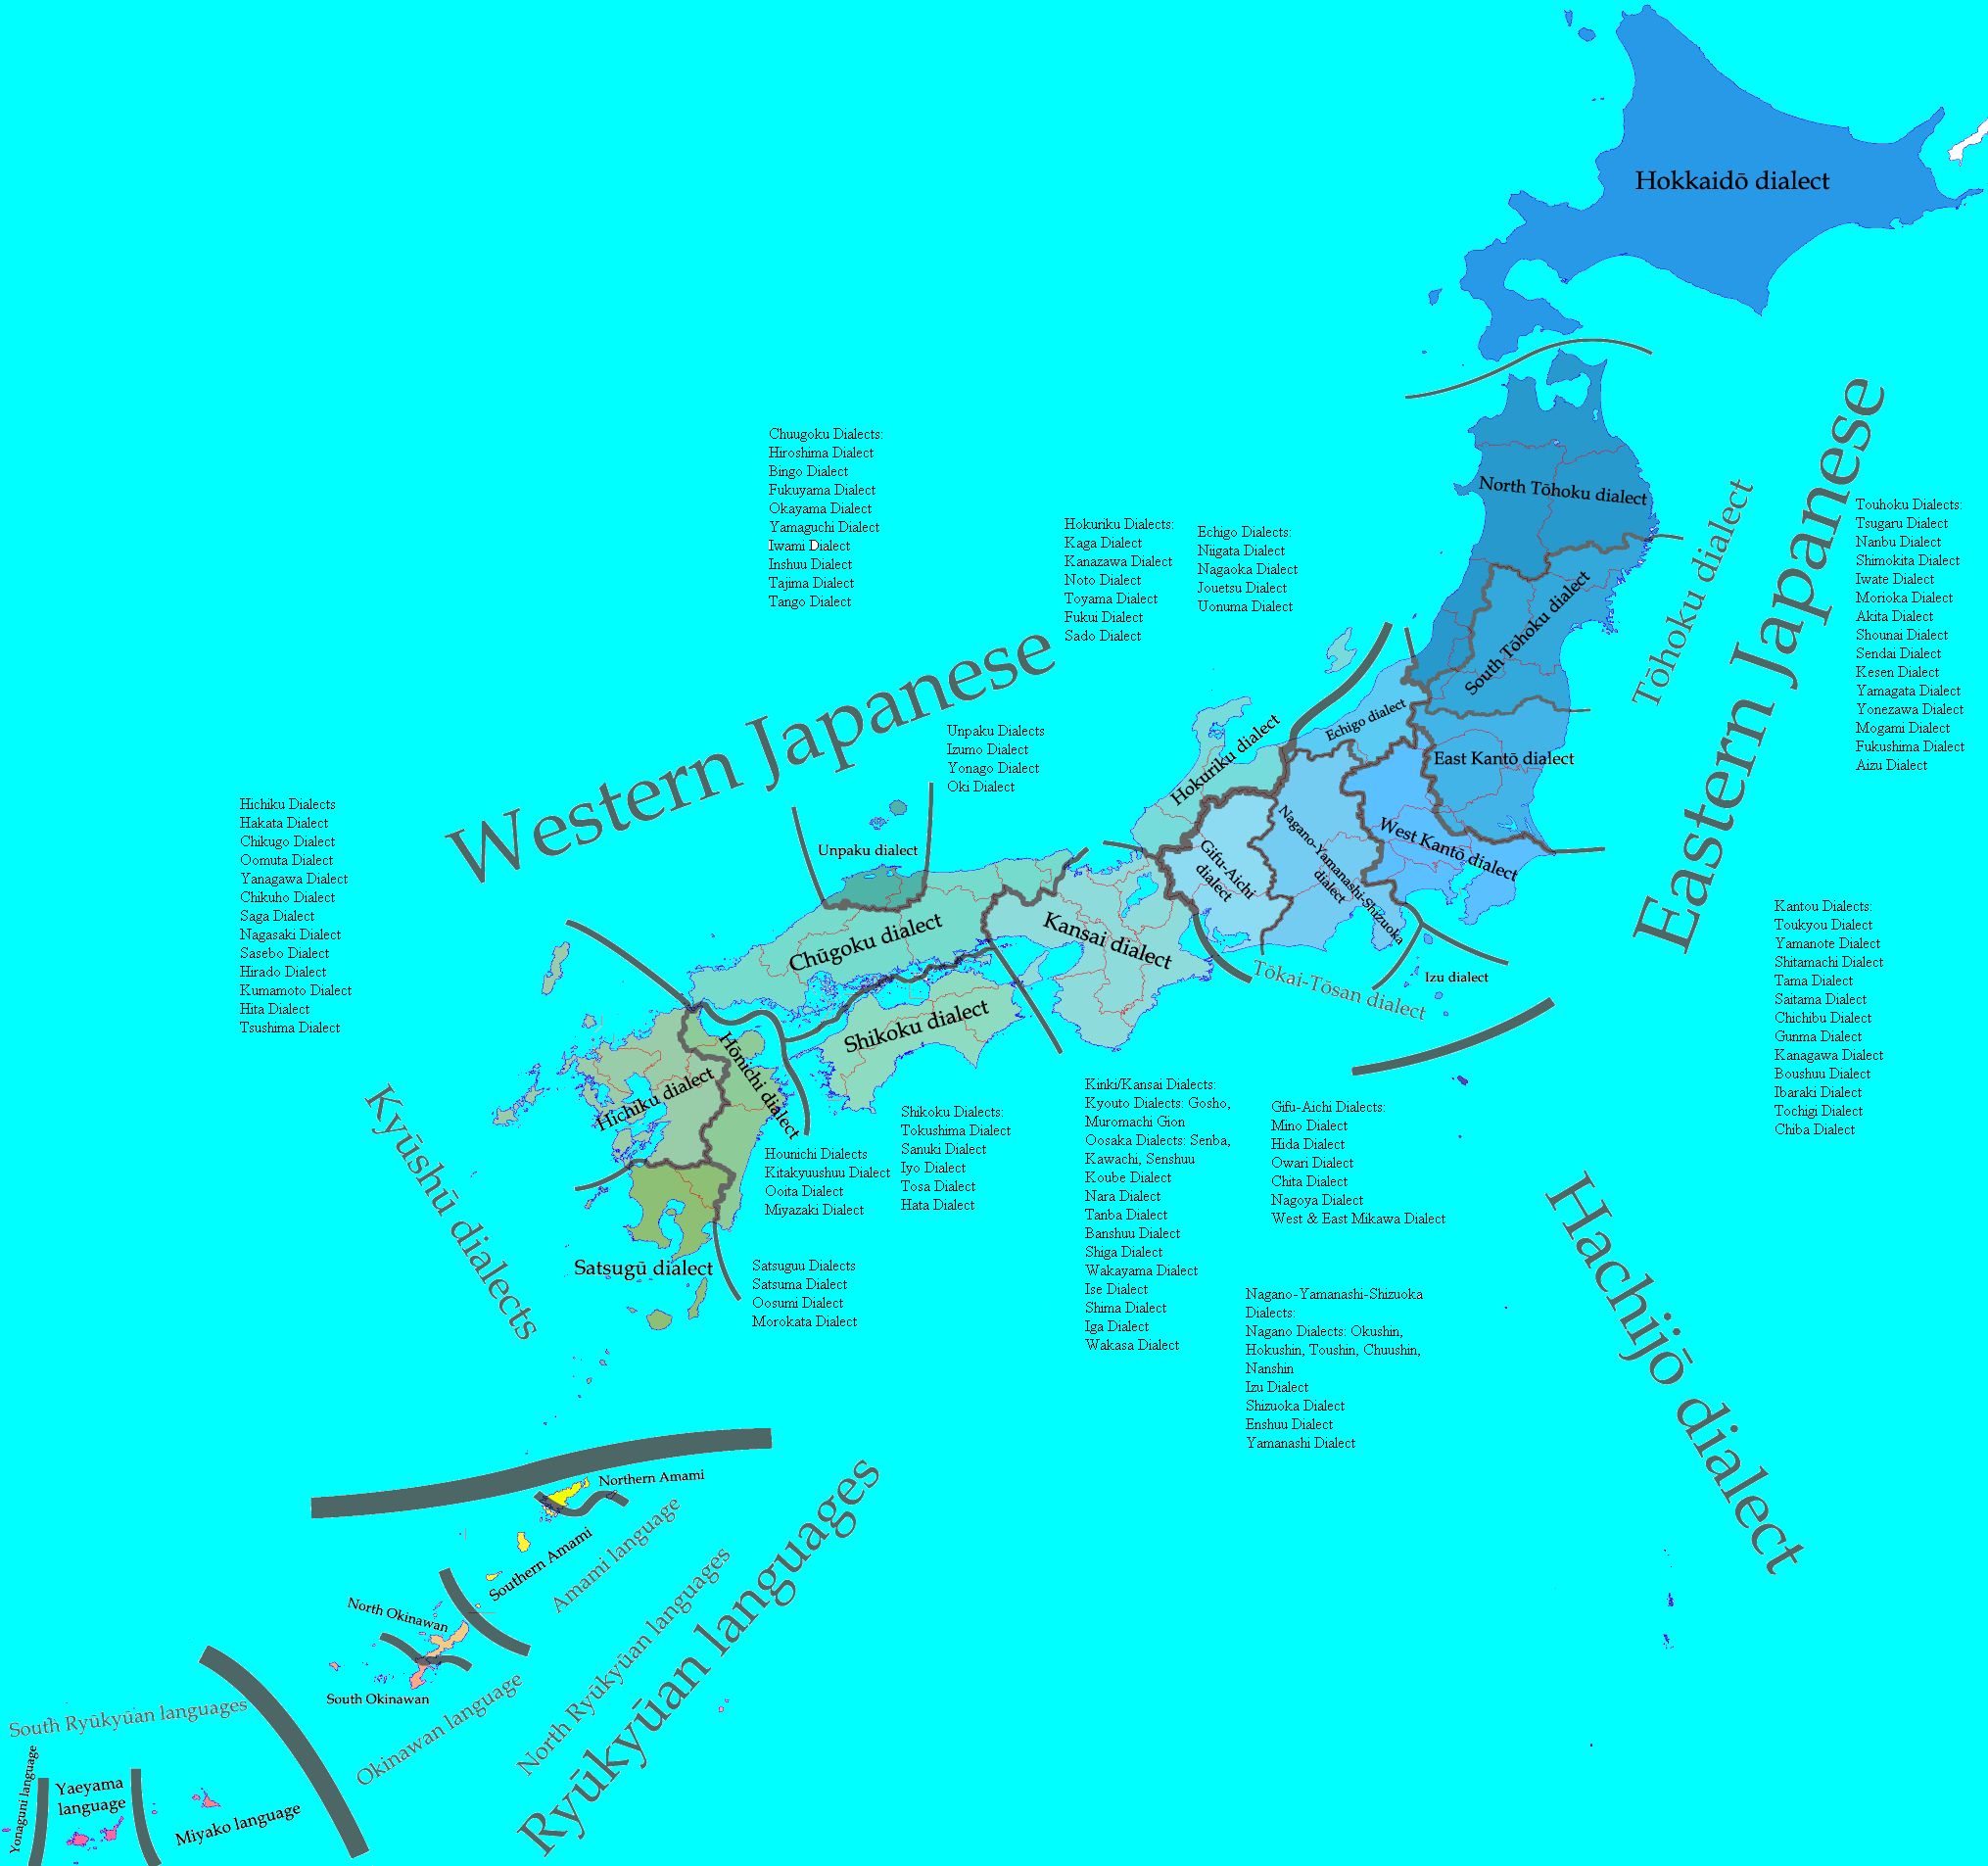
\includegraphics[width=0.9\textwidth]{figs/第01章/第7課:_10majoraspects_fig/Japanese_dialects.png}

\end{figure}
 
\par{ Dialects may differ in vocabulary, grammar, and punctuation. However, the most important dialect is Standard Japanese. By mastering this dialect, you will be able to converse with essentially any native Japanese speaker. Knowing other dialects is not essential to speaking or understanding Japanese, but many dialectal expressions are known by all spea kers. Whenever you watch anime or read manga, you will frequently encounter other major dialects. With this being the case, occasional focus will be given to dialectal expressions that are too important to ignore. }
    